\documentclass[MScCS]{uccthesis}
\usepackage[hidelinks]{hyperref}
\usepackage{graphicx} 
\usepackage{tcolorbox}
\usepackage{tabularx}
\usepackage{float}

\usepackage{csquotes} % Needed for biblatex
\usepackage{biblatex} %Imports biblatex package
\addbibresource{mybib.bib}

\setlength{\parskip}{1em}  % Adjusts space between paragraphs
\setlength{\parindent}{0pt}  % Removes paragraph indentation (optional)

\title{Analysis of mobile network coverage for vehicular traffic on Irish roads}
\author{Yugansh Nilesh Suryavanshi}
\supervisor{Professor Cormac Sreenan}
\secondreader{Dr Aisling O'Driscoll}
\date{\today}

\newcommand*{\COMMAND}[1]{\texttt{\textbackslash #1}}
\newcommand*{\COMMANDWITHARGUMENT}[2]{\texttt{\textbackslash #1}\{#2\}}




\abstract{%
   The rapid development and progress of mobile telecommunications technology has fundamentally transformed connectivity requirements along major transportation corridors. In Ireland, the deployment of 4G and 5G networks represent essential growth in infrastructure supporting economic growth and digital transformation. However, there are some significant gaps in understanding how network performance varies spatially and temporally along major transportation corridors, such as the M7 Dublin to Limerick motorway and N40 Cork Ring Road, where factors such as distance, seasonal weather patterns, and traffic congestion can greatly impact network performance.

   This research has used a detailed mixed-methods approach that combines quantitative spatial analysis of real ComReg ( Commission for Communications Regulation) coverage data with temporal analysis of TII (Transport Infrastructure Ireland) traffic patterns. The study analyzed 12,238 geographic points (11,108 M7 points, 1,130 N40 points) across two major Irish motorways, comparing traditional Hata Cost-231 models with 3GPP TR 38.901 standardized models for 4G and 5G networks. Advanced spatial clustering techniques (K-means and DBSCAN) were applied to identify coverage patterns and network complementarity. The methodology integrated real-world coverage measurements from Vodafone and Three networks with hourly traffic data from 29 monitoring sites, enabling correlation analysis between network performance and traffic patterns.

   The analysis revealed an overall coverage rate of 98.9\% across 12,238 locations, with significant variations between networks and roads. M7 demonstrated coverage percentages of 98.2\% (Vodafone 4G), 68.6\% (Vodafone 5G), 99.0\% (Three 4G), and 96.2\% (Three 5G), while N40 achieved consistent 97.3\% coverage across all networks. Model comparison analysis showed Hata models predicting approximately 98\% coverage while 3GPP models predicted  77\% coverage, resulting in a 78.6\% agreement between the two models. Temporal analysis revealed peak traffic hours (16:00) with M7 averaging 1,496 vehicles/hour (peak: 2,766 vehicles) and N40 averaging 2,877 vehicles/hour (peak: 5,628 vehicles), showing peak-to-average ratios of 1.85 and 1.96 respectively. Network reliability analysis showed 98.4\% operator overlap on M7 and 100\% on N40, with both roads demonstrating mature 4G-5G transition patterns. Seasonal analysis identified Spring 2025 as peak season (1.11x factor) and Summer 2024 as lowest (0.75x factor). These findings provide evidence-based insights for infrastructure planning and capacity optimization in Ireland's mobile telecommunications sector, supporting informed decision-making for network densification and 5G deployment strategies.

}

%\dedication{%
%   Your dedication here.
%}

%\acknowledgement{%
%   Your acknowledgement here.
%}

\renewcommand\addToFrontMatter[0]{%
}

\begin{document}
  \chapter{Introduction}

\section{Research Background}

The evolution of mobile telecommunications from 4G to 5G has fundamentally transformed how societies communicate, work, and access information. High-speed mobile connectivity is now recognized as critical infrastructure for economic growth and digital transformation \cite{eu2016_action_plan}. In Ireland, extensive deployment of 4G networks and the ongoing rollout of 5G represent major investments to enhance connectivity across both urban and rural areas. National policy targets reflect this importance: "Ireland's Digital Connectivity Strategy aims to cover all populated areas with 5G service by 2030" \cite{decc2022_strategy}.

The M7 motorway (Dublin-Limerick) and the N40 Cork ring road offer ideal case studies for mobile network performance, as these routes carry heavy traffic through diverse terrains (urban, suburban, and rural) and thus exemplify the connectivity challenges along transportation corridors. Ensuring reliable mobile coverage on such corridors is not only vital for commuters and businesses, but also a strategic objective at the European level---"the EU's 5G Action Plan calls for uninterrupted 5G coverage along main transport paths by 2025." \cite{eu2016_action_plan}.

Analyzing mobile network coverage has become increasingly complex with the introduction of 5G technology. Unlike 4G, which primarily operates in bands below 2.6GHz, 5G New Radio can utilize mid-band and millimeter-wave frequencies that enable higher capacity and data rates but suffer from shorter propagation ranges and greater susceptibility to environmental obstacles \cite{tsoulos2024highway}. Accurately modeling signal propagation at these higher frequencies requires more sophisticated approaches than the traditional macrocell models used for 4G network planning.

Classic empirical models like the Hata formula and its COST-231 extension provide simple predictions of path loss in mobile networks, but they assume average terrain and clutter conditions and were originally tuned for earlier cellular systems up to 2GHz \cite{hata1980empirical, cost231}. In contrast, modern standardized models capture the 3D propagation effects and frequency-dependent phenomena that characterize 4G and 5G channels. The 3GPP's study on LTE channel models (TR36.873) introduced geometry-based stochastic modeling for urban macrocells \cite{3gpp_tr36873}, and the 5G channel model (TR38.901) extends this to frequencies up to 100 GHz with detailed subpath, blockage, and spatial consistency parameters \cite{3gpp2024channel}.

The Commission for Communications Regulation (ComReg) in Ireland provides an excellent resource for studying these issues in a real-world context. ComReg maintains comprehensive nationwide coverage maps based on operator data and measurements, which classify signal quality into standardized categories (Very Good, Good, Fair, Fringe, No Coverage) as defined in technical guidelines \cite{comreg_plum_21118}. These rich datasets, combined with the availability of Transport Infrastructure Ireland (TII) traffic statistics for national roads \cite{tii2024indicators}, enable advanced research into how new 5G propagation models compare to legacy models and how coverage varies across geography and time in an Irish setting.

\section{Problem Statement}

Despite significant investments in mobile infrastructure, a critical gap remains in understanding how network performance varies both spatially and temporally along major transportation corridors. Most coverage analysis focus on static, aggregate metrics---for example, population coverage percentages or snapshots of signal strength---which can fail to capture the dynamic nature of mobile usage on busy roadways. Along motorways and ring roads, network demand and performance can fluctuate rapidly due to changing traffic volumes, diverse topographical features, and intermittent obstacles \cite{tsoulos2024highway}.

In Ireland, this limitation is particularly pronounced given the mix of densely populated corridors and expansive rural stretches. The M7 traverses open countryside and varied terrain in the Midlands, while the N40 navigates an urban environment with complex radio propagation conditions. Varying terrain and seasonal weather can significantly impact signal propagation and reliability along these routes, yet these effects are not fully accounted for in conventional planning models.

Empirical studies have only begun to scrutinize high-speed travel environments; recent field measurements on European motorways show that geography and infrastructure along a route can cause pronounced fluctuations in signal strength and quality \cite{tsoulos2024highway}, underscoring the need for more granular corridor-specific analysis.

Another challenge lies in accurately predicting coverage quality during the transition from 4G to 5G networks. While 5G promises enhanced capacity and lower latency compared to 4G \cite{tsoulos2024highway}, realizing these benefits in practice requires dense infrastructure and robust propagation models. 5G New Radio deployments in many countries initially use Non-Standalone (NSA) architecture, piggybacking on 4G LTE anchors. This means that 4G and 5G systems must coexist and hand off seamlessly, and coverage experienced by users results from a combination of both networks.

The higher-frequency 5G signals, weaken the signal strength faster with distance and are more easily blocked by obstacles than 4G's lower frequencies. Simplified propagation models---such as the Hata/COST-231 model widely used for macrocell coverage planning---do not explicitly account for phenomena like frequency-dependent penetration loss, fast-fading spatial correlation, or the fine-grained diffraction effects that are important at 5G frequencies. Current planning methodologies in industry often still rely on these empirical models or overly general vendor recommendations, which may not adequately represent real-world conditions on complex routes.

In summary, the problem motivating this research is twofold: 
(1) A lack of detailed understanding of spatial and temporal coverage performance along key Irish roads, and 
(2) A need to evaluate and improve propagation modeling for the 4G--5G transition in real-world corridor environments.

\section{Research Questions}

This research addresses five specific questions organized into three thematic areas:

\textbf{Spatial Coverage Analysis}
\begin{enumerate}
\item What is the spatial distribution and coverage performance of 4G and 5G mobile networks along Ireland's major transportation corridors, specifically the M7 Dublin-Limerick motorway and N40 Cork Ring Road?

\item How do different network operators (Vodafone and Three) perform in terms of coverage reliability and network complementarity across these transportation corridors?
\end{enumerate}

\textbf{Technology Transition Analysis}
\begin{enumerate}
\setcounter{enumi}{2}
\item What is the current state of 4G to 5G technology transition along Irish motorways, and how does this transition vary between urban (N40) and inter-urban (M7) transportation corridors?

\item How accurately do traditional empirical models (Hata) and modern standardized models (3GPP) predict mobile network coverage performance in transportation corridor environments?
\end{enumerate}

\textbf{Temporal and Capacity Analysis}
\begin{enumerate}
\setcounter{enumi}{4}
\item What are the temporal traffic patterns and peak demand characteristics along the M7 and N40 corridors, and how do these patterns influence network capacity requirements?
\end{enumerate}

\section{Research Significance}

This research is significant from both the academic and the real-world perspective of telecommunications planning. From an academic perspective, it contributes to the growing body of literature on 5G network performance in non-urban settings. Early 5G research and trials have tended to focus on city environments or controlled testbeds; by contrast, this study provides insights into how 4G and 5G networks perform in a highway/motorway context, which has been less scrutinized compared with urban environments \cite{tsoulos2024highway}.

The findings will enrich our understanding of propagation behavior and network dynamics in high-mobility scenarios. Furthermore, the study's comparative evaluation of an established empirical model against latest-standard models offers a valuable validation of whether legacy tools are still adequate for current networks. The use of advanced analytical methods (such as GIS-based spatial analysis and clustering) also demonstrates how techniques from data science can be applied in telecom research to uncover patterns that might be missed by traditional averaging or coarse metrics.

Practically, the research provides evidence-based insights that can directly inform network planning, optimization, and policy in Ireland's telecommunications sector. Mobile operators can leverage the detailed coverage maps and performance statistics along the M7 and N40 to optimize their radio access networks. The comparison of models has infrastructure planning implications as well: if simple models are overestimating coverage on certain road segments, planned service upgrades might be insufficient unless models are corrected.

For regulators like ComReg, the results offer an independent assessment of coverage map accuracy and can support the setting of realistic coverage targets or thresholds for 5G. The timing analysis is also significant: it suggests that capacity planning should ensure sufficient cell throughput during peak traffic hours, and that any performance degradations at these times are identified and addressed.

In broader terms, this thesis supports Ireland's digital transformation goals and connectivity policies. Consistent with the aims of Ireland's National Broadband Plan and Mobile Phone \& Broadband Taskforce, it provides data-driven evidence to guide infrastructure investment decisions in rural and transportation settings \cite{dcenr2012nbp}. The methodology and findings are likely transferable to other regions and countries with similar geography or network deployment stages, meaning the work can serve as a reference for studies of mobile network performance in transportation corridors elsewhere.

\section{Research Context}

This research is situated within the context of Ireland's ongoing initiatives in telecommunications advancement and the wider European digital agenda. Ireland has explicitly recognized the importance of robust digital infrastructure as a foundation for economic and social development. The National Broadband Plan (NBP) launched in 2012 set out to deliver high-speed internet to every part of Ireland, particularly addressing the urban-rural digital divide \cite{dcenr2012nbp}. While the NBP primarily focuses on fixed broadband, its overarching goal of a ``Connected Society'' complements the need for strong mobile coverage, since mobile networks are a key delivery mechanism for connectivity on the move.

In the mobile domain, the Department of Environment, Climate and Communications (DECC) published a Digital Connectivity Strategy in 2022 which reinforced targets for both fixed and wireless networks---including milestone goals for nationwide 5G coverage by 2030 \cite{decc2022_strategy}. This strategy aligns with the EU's vision for a Digital Decade by 2030, wherein digital infrastructures (like 5G corridors) are one of the central pillars \cite{eu2016_action_plan}.

Regulatory and industry context is also important to understanding this research. ComReg, as Ireland's communications regulator, has actively facilitated the rollout of advanced mobile services, for example, through spectrum auctions and coverage obligations. The multi-band spectrum award in 2021 (ComReg Document 21/40) released new spectrum in the 700MHz, 2.1GHz, 2.3GHz, and 2.6GHz bands to operators, enabling operators like Vodafone, Three, and Eir to expand 4G capacity and deploy 5G \cite{comreg2140_IM}. ComReg also provides public transparency tools---its Outdoor Coverage Map allows consumers and researchers to examine the reported coverage for every operator at any location \cite{comreg2022coveragemap}.

Meanwhile, TII (Transport Infrastructure Ireland) continually monitors traffic patterns on national roads and publishes statistics such as Annual Average Daily Traffic and real-time traffic counts \cite{tii2024indicators}. By combining these cross-sector data sources (telecom and transport), this research sits at the intersection of telecommunications engineering and transport geography, reflecting a multidisciplinary context. It acknowledges that connectivity is not only a telecom issue but also an enabler for smart transportation systems and public safety on roads.

The research thus takes place at a pivotal moment when insights into coverage and performance can feed into the next cycle of network enhancements---such as the move toward 5G Standalone networks, the planning of 6G trials, or the development of connected vehicle infrastructure. By grounding the analysis in real data and aligning it with Ireland's strategic goals, this thesis contributes both to scholarly discourse and to the practical roadmap for Ireland's digital connectivity future.


\chapter{Literature Review}

\section{Technologies, Libraries and Tools}

\subsection{Path-loss Models}

This thesis uses a mix of classical and standards-based radio models to benchmark measured signal levels along Irish motorway corridors.

Hata (1980) and COST-231 Hata provide fast, empirically derived path-loss estimates long used for macrocell planning at sub-2 GHz \cite{hata1980empirical, cost231}. Hata's original work defines suburban/urban correction factors and median loss formulas widely reproduced in planning texts.

3GPP TR 38.901 generalizes to modern 4G/5G bands (0.5--100 GHz) and scenarios (UMa/UMi/RMa) with frequency-dependent formulas and statistical channel parameters used in system-level simulations \cite{3gpp2024channel}. The specification is regularly updated by 3GPP with new releases that incorporate the latest research and industry requirements.

ITU-R P.1812-6 (2021) is used for point-to-area predictions in the 30 MHz--6 GHz range and is helpful where terrain/clutter dominate (long rural paths). The official entry notes says ``A path-specific propagation prediction method for point-to-area terrestrial services in the frequency range 30 MHz to 6 000 MHz.'' \cite{itu_p1812_6}.

 Hata/COST-231 offer transparent baselines but can need local calibration; 38.901 and P.1812 provide scenario- and path-specific structure better aligned to 5G macro at 3.5 GHz and Irish topography.

\subsection{Data sources used for coverage and demand}

ComReg drive-test and public tools : The Siteviewer / Base-Station map helped provide a better understanding of the existing network layout. \cite{comreg_base_stations, comreg2022coveragemap}.

TII National Roads Network Indicators 2023 : Referred to better understand the volumes of Annual Average Daily Traffic (AADT) and hourly profiles along the M7 and N40, This Transport Infrastructure Ireland report provides official counts and indicators \cite{tii2024indicators}.

ComReg market statistics (QKDR) : The 2025 ``25/13 -- This Quarterly Key Data Report helped by providing market statistics about Irish mobile network usage, subscriber numbers, and industry trends.\cite{comreg25_13}.

OpenStreetMap Overpass API : The official user manual and OSM wiki gave the QL syntax and examples which helped to get lat/lon coordinates for the highways. \cite{osm_overpass}.

\subsection{Python geospatial \& ML stack}

\textbf{NumPy:} NumPy underpins array math used across all pipelines \cite{harris2020array}. The library provides efficient multi-dimensional array operations and mathematical functions that form the computational foundation for all data processing tasks in this research, including signal strength calculations and statistical analysis.

\textbf{Pandas:} Pandas is used for tabular ETL and time-series handling \cite{mckinney2017python}. The library offers powerful data manipulation capabilities for structured data, enabling efficient processing of coverage measurements, traffic data, and temporal analysis. Its time-series functionality is particularly valuable for analyzing hourly and daily traffic patterns along the motorways.

\textbf{GeoPandas:} GeoPandas enables GIS operations (GeoDataFrame/GeoSeries) and mapping. The library provides detailed documentation and API references that describe the spatial data structures and geometric operations used in this research \cite{jordahl2020geopandas}. It extends pandas with spatial capabilities, allowing for coordinate system transformations, spatial joins between coverage points and road segments.

\textbf{Scikit-learn:} Scikit-learn provides KMeans and DBSCAN for spatial/temporal clustering \cite{pedregosa2011scikit}. The library implements machine learning algorithms for identifying coverage patterns and traffic clusters. K-means is used for partitioning coverage areas into quality groups, while DBSCAN identifies irregularly shaped coverage clusters and detects locations with poor signal strength.

\section{Prior Studies}

\subsection{Highway 4G/5G measurement studies}

Highway-scenario field work (3.5 GHz). Tsoulos et al. analyze 5G vs 4G on highways, documenting blockage and shadowing dynamics and offering empirical comparisons; they conclude 5G highway performance is environment-sensitive and quantify differences to LTE \cite{tsoulos2024highway}.
This study conducts real vehicular measurements in the exact scenario class relevant here.
It was implemented for the National Highway of (Greece), and results may not transfer to Irish rural morphology.


\subsection{Rural coverage improvement literature}

Cabrera-Castellanos et al: (2021) survey rural with ``not-spot'' solutions (small cells, satellites, UAV relays) and policy targets (e.g., UK 95\% targets). The study provides a comprehensive overview of available technologies and deployment options. However, it focuses on general rural areas rather than specific transportation corridors and offers high-level synthesis rather than detailed implementation analysis \cite{Cabrera2021}.

Policy \& programmes : The EU's 5G Action Plan set early corridor ambitions \cite{eu2016_action_plan}, and funding selects cross-border trials (e.g., 5GCroCo) to support connected mobility \cite{5gcroc_project}. These documents establish corridors as a policy priority but are programmatic rather than measurement-based.

The current research differs by focusing on every geographic segment of the highways and analyzing what percentage of the highways has adequate coverage.

\subsection{Irish road coverage context}

ComReg/Oxera (2018) examined how population coverage obligations map to roads, highlighting costs and practical measures to accelerate roll-out (e.g., ducts) \cite{comreg2018improving}. This represents the first Ireland-specific bridge from population to roads coverage analysis. However, the approach is model-driven rather than based on high-resolution measurements.

ComReg/Plum coverage thresholds (2021) : Plum's technical study proposed coverage categories and thresholds to map radio frequency (RF) metrics to consumer-friendly labels \cite{comreg_plum_21118}. The study provides defensible thresholding and key performance indicators (KPI)-to-class mapping methodology. However, these thresholds would benefit from empirical validation in specific environments. The current research explicitly validates these categories on measured motorway data.

\begin{table}[h]
   \centering
   \begin{tabular}{|l|c|c|c|}
   \hline
   \textbf{Coverage Quality} & \textbf{4G RSRP (dBm)} & \textbf{5G SS-RSRP (3.5 GHz)} & \textbf{Service Description} \\
   \hline
   Very Good & -85 or stronger & -97.4 or stronger &  Maximum data speed \\
   \hline
   Good & -85 to -95 & -97.4 to -107.4 & Good data speeds \\
   \hline
   Fair & -95 to -105 & -107.4 to -117.4 &  Marginal data speeds  \\
   \hline
   Fringe & -105 to -115 & -117.4 to -127.4 & Poor data speeds \\
   \hline
   No Coverage & Below -115 & Below -127.4 &  No coverage  \\
   \hline
   \end{tabular}
   \caption{ComReg Plum Consulting coverage quality thresholds (Table 1 and Table 6.1)}
   \label{tab:plum_coverage_thresholds}
   \end{table}



ComReg 21/40 (2021) spectrum award IM : Provides the spectrum framework that underpins 4G/5G capacity on Irish networks \cite{comreg2140_IM}. Useful for capacity context on motorway corridors.

The current research combines the Plum thresholds with field measurements and clustering to test if public coverage classes match ground truth along M7/N40.



\subsection{Spatial clustering for coverage analysis}

DBSCAN \& K-means fundamentals: DBSCAN \cite{ester1996} detects arbitrarily-shaped dense regions and flags outliers; K-means \cite{macqueen1967} provides simple partitioning given a chosen k. 

Telecom applications: Margaris et al. show that hybrid clustering (including a hierarchical DBSCAN) improved 5G KPI spatial segmentation---useful when coverage patterns deviate from convex shapes \cite{margaris2022hybrid}.

Identifying weak coverage: Li \& Peng (2022) combined signal strength and spatial proximity to cluster weak-coverage regions with DBSCAN, a conceptual precedent for the ``fringe/poor segment'' delineation used in this research \cite{Li2022}.


\subsection{Traffic clustering and demand alignment}

Eftekhar et al. (2023) cluster daily travel-production patterns in the Netherlands, showing stable within-day profiles linked to urbanization \cite{Eftekhar2023}. The study provides interpretable daily profiles but focuses on transport rather than telecom KPIs.

Broader traffic literature shows time-series clustering supporting forecasting and detector grouping (e.g., K-means/GRU hybrids, spatio-temporal clustering). These reinforce the idea of profile-based site grouping used here. The GeoPandas library documentation explains the two primary methods for combining datasets: attribute joins and spatial joins. These techniques are leveraged to integrate traffic sites with coverage segments \cite{jordahl2020geopandas}.


\subsection{Market and MVNO context}

ComReg 22/72 lists MVNOs using Three's network (e.g., 48, Lyca), clarifying why analyzing Three's network and services provided can proxy for multiple retail brands in corridor results \cite{mvnodetails_three_ie}.

\begin{center}
\fbox{\parbox{0.95\textwidth}{
\textbf{Key Note:} An MVNO is a company that provides mobile phone services to customers but doesn't own the actual network infrastructure. Instead, they rent network capacity from the main network operators.
}}
\end{center}

\subsection{European corridor initiatives}

EU 5G corridors policy frames cross-border routes for connected mobility; CORDIS projects such as 5GCroCo are representative testbeds \cite{eu2016_action_plan, 5gcroc_project}.

Operator programmes. Vodafone Germany's plan to add $\sim$150 5G sites along Autobahns underscores the trend toward road-focused rollouts; the RCR Wireless report captures the announcement \cite{vodafone_autobahn}.

\section{Synthesis}

\begin{itemize}
\item \textbf{Empirical, corridor-specific validation:} Most prior work is either high-level policy (EU/ComReg) or campus/urban trials. This study grounds motorway coverage with $>$12k measured points and official traffic counts.

\item \textbf{Dual-model benchmarking:} Direct COST-231 Hata vs 3GPP TR 38.901 comparison on the same Irish highways is rare and reveals environment-specific bias.

\item \textbf{Cluster-of-coverage:} Using K-means and DBSCAN algorithms to analyze coverage measurements reveals distinct quality zones and identifies areas requiring network improvement attention.

\item \textbf{Ireland-specific regulatory context:} This research validates ComReg/Plum thresholds against real measurements and situates results in the spectrum and market structure (21/40, QKDR, MVNOs).
\end{itemize}


\chapter{Methodology}

   \section{Research Design}

   \subsection{Overall Approach}
   This research employes a mixed-methods approach by combining the quantitative spatial analysis of coverage data using real ComReg measurements, temporal analysis of traffic patterns using TII data, statistical validation of path loss models with quantified accuracy metrics, advanced clustering and complementarity analysis, and capacity planning assessment with verified parameters. The analytical workflow was implemented using Python and modern data science tools, including NumPy and Pandas for data handling \cite{harris2020array,mckinney2017python}, GeoPandas and PySAL for spatial analysis \cite{jordahl2020geopandas,Rey2007}, and scikit-learn for machine learning tasks \cite{pedregosa2011scikit}.

   \subsection{Data Sources}
   The analysis utilized real coverage data from the Commission for Communications Regulation (ComReg):
   \begin{itemize}
   \item M7 Motorway: 11,108 coverage sample points
   \item N40 Cork Ring Road: 1,130 coverage sample points
   \item Four networks: Vodafone 4G/5G, Three 4G/5G
   \item Coverage quality levels: Very Good, Good, Fair, Fringe, No Coverage
   \item Data collection period: May-June 2025
   \end{itemize}

   Real traffic data was obtained from Transport Infrastructure Ireland (TII) :
   \begin{itemize}
   \item M7 Motorway: 504 traffic records from 21 sites
   \item N40 Cork Ring Road: 192 traffic records from 8 sites
   \item Date range: May 1, 2025 to June 4, 2025
   \item Hourly traffic patterns and volume data
   \item Weekday vs weekend traffic analysis
   \end{itemize}

   

   \textbf{Network Provider Coverage:} While the primary analysis focuses on Vodafone and Three networks, the findings effectively extend to four service providers. Lyca Mobile and 48 Mobile operate on Three's network infrastructure, meaning our analysis of Three's network performance directly applies to these additional providers \cite{mvnodetails_three_ie}. This provides comprehensive coverage of Ireland's major mobile service providers.
   
   


   \subsection{Highway Selection}
   The selection of M7 and N40 motorways was strategically designed to enable generalization of findings across different types of Irish road networks:

   \textbf{M7 Dublin-Limerick Motorway:} Selected as a representative long-distance, inter-urban highway connecting Ireland's capital to a major regional city. This 166-kilometer motorway traverses diverse geographic terrain including urban, suburban, and rural environments, making it ideal for comprehensive spatial coverage analysis. The M7 serves as a model for other major inter-urban routes such as M1 (Dublin-Belfast), M4 (Dublin-Galway), and M8 (Dublin-Cork).

   \textbf{N40 Cork Ring Road:} Chosen as a representative urban ring road providing circumferential connectivity around Ireland's second-largest city. This 17-kilometer expressway experiences high traffic density and complex urban propagation conditions, making it perfect for detailed temporal traffic pattern analysis. The N40 serves as a model for other urban ring roads and high-capacity urban corridors across Ireland.

   This dual approach enables findings to be generalized across both long-distance inter-urban highways and urban ring roads, providing comprehensive insights for Ireland's diverse road network infrastructure.


   \begin{figure}[htbp]
   \centering
   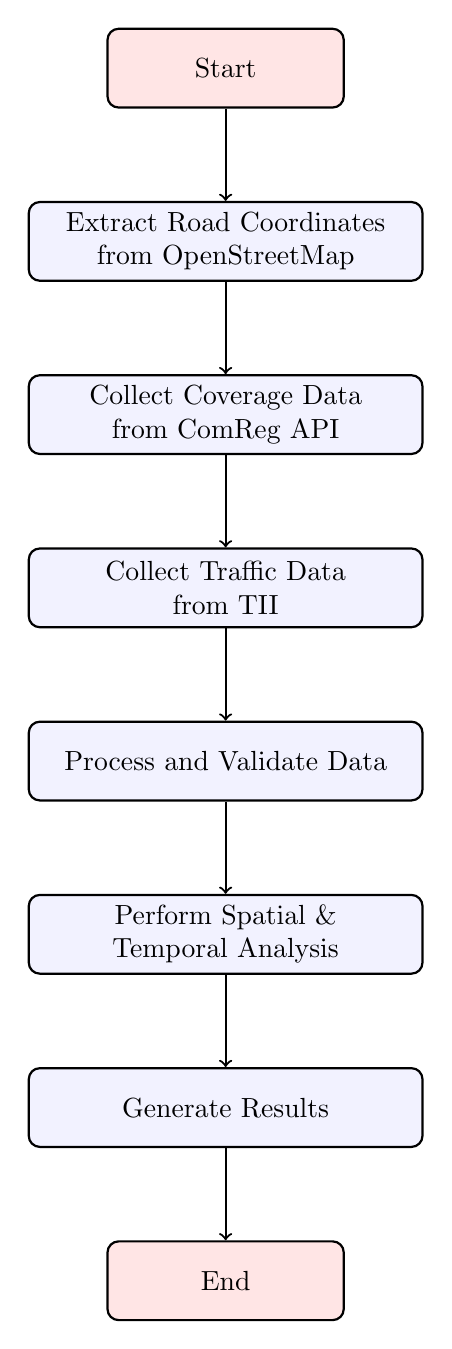
\begin{tikzpicture}[
       node distance=2.2cm,
       startstop/.style={rectangle, draw=black, thick, minimum width=3cm, minimum height=1cm, align=center, fill=red!10, rounded corners=4pt},
       process/.style={rectangle, draw=black, thick, minimum width=5cm, minimum height=1cm, align=center, fill=blue!5, rounded corners=4pt},
       arrow/.style={->, thick, black}
   ]
   \node[startstop] (start) {Start};
   \node[process, below of=start] (osm) {Extract Road Coordinates\\from OpenStreetMap};
   \node[process, below of=osm] (comreg) {Collect Coverage Data\\from ComReg API};
   \node[process, below of=comreg] (tii) {Collect Traffic Data\\from TII};
   \node[process, below of=tii] (process) {Process and Validate Data};
   \node[process, below of=process] (analyze) {Perform Spatial \&\\Temporal Analysis};
   \node[process, below of=analyze] (results) {Generate Results};
   \node[startstop, below of=results] (end) {End};

   \draw[arrow] (start) -- (osm);
   \draw[arrow] (osm) -- (comreg);
   \draw[arrow] (comreg) -- (tii);
   \draw[arrow] (tii) -- (process);
   \draw[arrow] (process) -- (analyze);
   \draw[arrow] (analyze) -- (results);
   \draw[arrow] (results) -- (end);
   \end{tikzpicture}
   \caption{Data collection and analysis workflow}
   \label{fig:data_flow}
   \end{figure}

   
   \section{Data Collection Methodology}

   \subsection{Geographic Data Collection}
   The research required precise geographic coordinates for the target road networks to enable systematic coverage data collection. The geographic coordinates for both motorways were obtained from OpenStreetMap (OSM), a collaborative mapping platform that provides detailed geographic data under the Open Database License (ODbL) \cite{osm_overpass}.

   \textbf{M7 Motorway Data:}
   \begin{itemize}
   \item Source: OpenStreetMap via Overpass API
   \item File: ireland\_highways.geojson
   \item Extraction Date: May 13, 2025
   \item Data Type: MultiLineString geometry with route properties
   \item Network: IE:motorway (Irish motorway network)
   \item Reference: M7 motorway route from Dublin to Limerick
   \item Coordinate Count: 11,108 points along the motorway route
   \item Sampling Interval: 50 meters between consecutive points
   \end{itemize}

   \textbf{N40 Cork Ring Road Data:}
   \begin{itemize}
   \item Source: OpenStreetMap via Overpass API
   \item File: cork\_ring\_road.geojson
   \item Extraction Date: July 30, 2025
   \item Data Type: LineString geometry with highway properties
   \item Highway Type: trunk road (N40 expressway)
   \item Reference: South Ring Road around Cork city
   \item Coordinate Count: 1,130 points along the ring road
   \item Sampling Interval: 50 meters between consecutive points
   \end{itemize}

\begin{center}
\fbox{\parbox{0.95\textwidth}{
\textbf{Please Note:}
ComReg's coverage mapping system utilizes a tile-based architecture that provides broad geographic coverage but lacks the granular precision required for highway-specific analysis. To overcome this limitation and obtain precise coverage data along transportation corridors, the research employed OpenStreetMap to extract geographic coordinates at 50-meter intervals along the M7 and N40 motorways. This approach generated 11,108 sampling points for the M7 Dublin-Limerick motorway and 1,130 points for the N40 Cork Ring Road, enabling targeted coverage data collection at specific highway locations rather than relying on general area-based tiles.
}}
\end{center}

   \subsection{Comreg Data Collection}
   The research employed an iterative approach to data collection, evolving from initial web scraping attempts to more robust API-based methodologies. This evolution was driven by technical challenges encountered during the initial implementation phase and the need for reliable, scalable data collection processes.

   \textbf{Initial Selenium Implementation:}
   The research initially attempted to utilize Selenium WebDriver for automated data collection from ComReg's coverage mapping system. Selenium was selected based on its widespread use in web automation and its ability to handle dynamic web content.

   \textbf{Technical Challenges Encountered:}
   The Selenium implementation encountered several significant challenges that necessitated a methodological shift:
   \begin{itemize}
   \item Anti-Automation Measures: ComReg's website implemented sophisticated bot detection mechanisms
   \item Session Management: Complex session handling requirements and frequent session invalidation
   \item Performance Limitations: Slow execution times due to browser rendering overhead
   \item Reliability Issues: Inconsistent success rates due to dynamic content loading
   \item Scalability Constraints: Difficulty in scaling to handle large numbers of coordinate points
   \end{itemize}

   \textbf{Transition to API-Based Methodology:}
   Based on the challenges encountered with Selenium, the research transitioned to an API-based approach for data collection. This transition was informed by research demonstrating the advantages of API-based data collection over traditional web scraping methods.

   \textbf{API Implementation Advantages:}
   The API-based approach provided significant advantages:
   \begin{itemize}
   \item Reliability: Consistent success rates with proper error handling
   \item Performance: Significantly faster execution times due to direct API communication
   \item Scalability: Ability to handle large datasets efficiently with concurrent requests
   \item Maintainability: Simplified codebase with reduced complexity
   \item Resource Efficiency: Lower computational requirements and reduced network overhead
   \end{itemize}


   \subsection{TII Data Collection Challenges}
   The collection of traffic data from Transport Infrastructure Ireland (TII) presented unique challenges that required a different approach compared to the ComReg data collection. Initial attempts to automate data collection from TII's traffic monitoring system encountered significant technical barriers.

   \textbf{403 Forbidden Error Encountered:}
   All automated access attempts resulted in HTTP 403 Forbidden errors, indicating that TII's server actively blocked automated access attempts. This response was consistent across different approaches:
   \begin{itemize}
   \item Direct HTTP Requests: All requests returned 403 Forbidden regardless of headers or authentication
   \item Session-Based Access: Attempts to establish persistent sessions were blocked
   \item Header Manipulation: Various user-agent and header modifications failed to bypass restrictions
   \item IP-Based Restrictions: Access was blocked regardless of request timing or frequency
   \end{itemize}

   \textbf{Manual Data Collection Strategy:}
   Upon encountering the 403 Forbidden errors, the research team conducted a comprehensive analysis of TII's website structure to understand the available data and develop an alternative collection strategy. The analysis revealed that TII provides comprehensive traffic data through manual download options on their website.

   
   \begin{figure}[htbp]
   \centering
   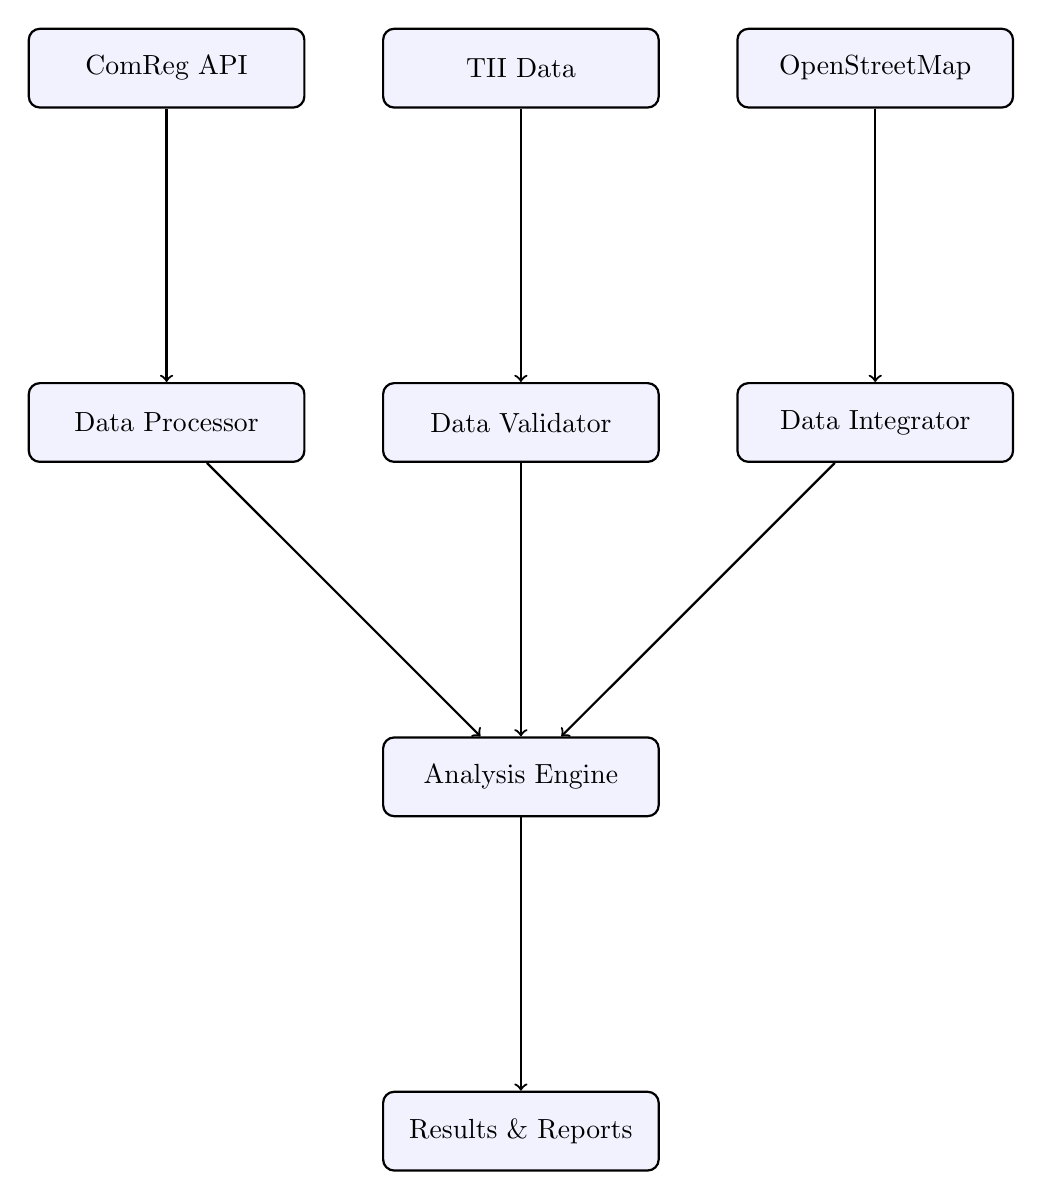
\begin{tikzpicture}[
       node distance=4.5cm,
       box/.style={rectangle, draw=black, thick, minimum width=3.5cm, minimum height=1cm, align=center, fill=blue!5, rounded corners=4pt},
       arrow/.style={->, thick, black}
   ]
   \node[box] (comreg) {ComReg API};
   \node[box, right of=comreg] (tii) {TII Data};
   \node[box, right of=tii] (osm) {OpenStreetMap};
   \node[box, below of=comreg] (processor) {Data Processor};
   \node[box, below of=tii] (validator) {Data Validator};
   \node[box, below of=osm] (integrator) {Data Integrator};
   \node[box, below of=validator] (analyzer) {Analysis Engine};
   \node[box, below of=analyzer] (output) {Results \& Reports};

   \draw[arrow] (comreg) -- (processor);
   \draw[arrow] (tii) -- (validator);
   \draw[arrow] (osm) -- (integrator);
   \draw[arrow] (processor) -- (analyzer);
   \draw[arrow] (validator) -- (analyzer);
   \draw[arrow] (integrator) -- (analyzer);
   \draw[arrow] (analyzer) -- (output);
   \end{tikzpicture}
   \caption{Data flow architecture showing data sources and processing}
   \label{fig:data_architecture}
   \end{figure}


  \section{Core Implementation}

  \subsection{Core Implementation Structure}
The project implementation consists of eight interconnected Python scripts organized into three functional categories, designed to provide a modular and scalable approach to mobile network coverage analysis. This architecture enables systematic data collection, processing, and analysis while maintaining code reusability and maintainability.

\subsection{Download Coverage Scripts }

The coverage data collection scripts (`M7\_Download\_Coverage.py`) and (`N40\_Download\_Coverage.py`)  implement automated data extraction from ComReg's coverage mapping API for the M7 Dublin-Limerick motorway and N40 Cork Ring road. The scripts serve as the primary data acquisition component for spatial analysis, providing comprehensive coverage quality metrics across multiple network operators and technologies.



\textbf{Technical Implementation:}
Both the scripts utilize ComReg's RESTful API to access the national coverage mapping database. The implementation includes robust error handling mechanisms, data validation protocols, and quality assurance checks to ensure reliable data collection.

\textbf{Data Collection Process:}
\begin{enumerate}
\item Initialize API connection with ComReg coverage mapping service
\item Load geographic coordinates for M7 motorway from OpenStreetMap data
\item Iterate every 50 meters to get 11,108 sampling points along the motorway
\item Extract coverage quality data for Vodafone 4G/5G and Three 4G/5G networks
\item Validate data quality and handle missing or erroneous entries
\item Store results in standardized JSON format with geographic coordinates
\end{enumerate}

\textbf{Output and Data Structure:}
The script generates a comprehensive JSON file containing coverage data with the following structure:

\begin{itemize}
\item \textbf{Geographic Coordinates:} Latitude and longitude for each sampling point
\item \textbf{Coverage Quality Metrics:} Quality classifications for each network operator and technology
\item \textbf{Data Validation Flags:} Quality indicators and validation status for each data point
\item \textbf{Metadata:} Collection timestamp, processing parameters, and data source information
\end{itemize}

\begin{center}
\fbox{\parbox{0.95\textwidth}{
\textbf{Please Note:} The coverage data collection phase utilized separate scripts for M7 highway and N40 motorway to ensure independent operation and fault isolation. While this approach resulted in some code duplication, it provided operational benefits including independent execution, road-specific optimization, and parallel development capabilities.
}}
\end{center}

\subsection{TII\_Data\_Processor.py}

The TII Data Processor script {TII\_Data\_Processor.py} implements comprehensive data processing of manually downloaded raw traffic data files from Transport Infrastructure Ireland for both M7 Dublin-Limerick and N40 Cork Ring Road motorways. This script serves as the primary data processing component for temporal analysis, providing comprehensive traffic pattern metrics across multiple temporal scales and monitoring sites.

\textbf{Technical Implementation:} The script employs automated HTML parsing techniques using BeautifulSoup to process manually downloaded TII data files stored in the local file system. The implementation includes robust error handling mechanisms, data validation protocols, and quality assurance checks to ensure reliable data processing across multiple file formats and temporal scales.

\textbf{Data Processing Process:}
\begin{enumerate}
\item Load manually downloaded raw TII files from local directories (M7: 21 sites, N40: 8 sites)
\item Process Daily Data: Extract hourly traffic patterns from daily TII files
\item Process Weekly Data: Analyze weekly traffic patterns and weekday/weekend variations
\item Process Monthly Data: Identify seasonal patterns and long-term trends
\item Process Multi-day Data: Handle extended period traffic analysis
\item Create Temporal Analysis: Integrate all temporal scales
\item Generate Data Quality Metrics: Validate data completeness and accuracy
\item Save Results: Create standardized outputs for analysis
\end{enumerate}


\textbf{Output and Data Structure:} The script generates two output files:
\begin{itemize}
\item \textbf{JSON Analysis File:} Contains aggregated statistics including total files processed, total records, total volume, total sites, and road comparison data
\item \textbf{Summary Report:} A text file with processing timestamp, total statistics, and per-road breakdown
\item \textbf{Console Output:} Real-time processing progress and final summary statistics
\end{itemize}



\section{Path Loss Modeling}

\subsection{Path Loss Model Implementation Methodology}

The research employed an iterative approach to path loss model implementation, evolving from initial evaluation of existing libraries to custom development from scratch. This evolution was driven by technical challenges encountered during the initial implementation phase and the need for Irish-specific parameterization and motorway corridor analysis requirements.

\textbf{Initial Library Evaluation:} The research initially attempted to utilize existing Python libraries and implementations for path loss modeling, including PyLayers \cite{pylayers2024} for COST-231 Hata models and AIMM Simulator \cite{aimm_simulator} for 3GPP TR 36.873 implementations. These libraries were selected based on their widespread use in academic research and their comprehensive coverage of standardized path loss models.

\textbf{Technical Challenges Encountered:} The library-based implementation encountered several significant challenges that necessitated a methodological shift:
\begin{itemize}
\item \textbf{Parameter Limitations:} Existing libraries lacked specific network parameters.
\item \textbf{Technology Coverage:} Incomplete implementation of both 4G and 5G models in single library solutions
\item \textbf{Customization Requirements:} Difficulty in modifying models for project-specific analysis needs
\item \textbf{Integration Complexity:} Challenges in integrating multiple libraries for proper analysis
\end{itemize}

\textbf{Transition to Custom Implementation:} Based on the challenges encountered with existing libraries, the research transitioned to custom implementation from scratch following 3GPP specifications \cite{3gpp_tr36873,3gpp_tr38901}. This transition was informed by research demonstrating the advantages of custom implementations for specific technical requirements.

This methodological evolution ensured that the path loss models were specifically tailored to the network conditions and project requirements, providing more accurate and relevant coverage predictions for the motorway analysis. The custom implementation approach, while requiring additional development effort, provided superior accuracy and relevance compared to generic library solutions.

\subsection{Hata Model Implementation}
   The Hata model was implemented with verified Irish parameters \cite{comreg25_13,itu_p1812_6}:
   
\begin{itemize}
\item Frequency: 1800 MHz for 4G (limited to frequencies up to 2 GHz)
\item Base station height: 30 meters (Irish planning guidelines)
\item Mobile station height: 1.5 meters (standard value)
\item EIRP: 67 dBm for 4G (ComReg verified)
\item Environment correction factor: 0 dB 
\item Maximum distance: 20 km
\end{itemize}

The model was implemented using the following formula :

\textbf{Path Loss:} 
\begin{equation}
\text{Path Loss (dB)} = 46.3 + 33.9 \times \log_{10}(f_{\text{MHz}}) - 13.82 \times \log_{10}(h_{\text{BS}}) - a_{hm} + (44.9 - 6.55 \times \log_{10}(h_{\text{BS}})) \times \log_{10}(d_{\text{km}}) + C_m
\end{equation}

Where:
\begin{itemize}
\item \textbf{a\_hm} = Mobile station antenna height correction factor
\item \textbf{C\_m} = Environment correction factor 
\item \textbf{frequency\_MHz} = Operating frequency in MHz (1800 for 4G)
\item \textbf{base\_station\_height} = Height of base station antenna in meters (30m)
\item \textbf{distance\_km} = Distance between base station and mobile device in kilometers
\end{itemize}

\begin{center}
\fbox{\parbox{0.95\textwidth}{
\textbf{COST-231 Hata Path Loss Formula:}
This formula calculates how much the radio signal weakens as it travels from the base station to the mobile device. It accounts for the frequency of the signal, the distance it travels, the heights of both antennas, and environmental factors. The logarithmic relationships reflect the real-world behavior of radio wave propagation, where signal strength decreases more rapidly at first and then more slowly as distance increases.
}}
\end{center}

   \subsection{3GPP Models Implementation}
   The 3GPP models were implemented according to \cite{3gpp2024channel,3gpp_tr36873}:
   \begin{itemize}
   \item 3GPP TR 36.873 for 4G LTE (Urban Macro scenarios)
   \item 3GPP TR 38.901 for 5G NR (UMa scenarios)
   \item Line-of-sight and non-line-of-sight conditions
   \item Irish-specific environmental factors
   \end{itemize}

   \subsubsection{3GPP 4G (TR 36.873) Formulas}
The 3GPP TR 36.873 model for 4G LTE was implemented using the following formulations:

\textbf{Breakpoint Distance:} d\_bp = 4 $\times$ h\_BS $\times$ h\_MS $\times$ f / c

\textbf{LOS Condition :}

Path Loss = 20 $\times$ log$_{10}$(4$\pi$ $\times$ distance $\times$ f / c) + min(0.03 $\times$ h\_e$^{1.72}$, 10) $\times$ log$_{10}$(distance) + min(0.044 $\times$ h\_e$^{1.72}$, 14.77) + 0.002 $\times$ log$_{10}$(h\_e) $\times$ distance

\textbf{NLOS Condition (distance > breakpoint):}
Path Loss = max(LOS\_path\_loss, NLOS\_component)

Where:
\begin{itemize}
\item \textbf{h\_BS} = Base station height (30m)
\item \textbf{h\_MS} = Mobile station height (1.5m)
\item \textbf{h\_e} = Effective environment height (1.0m)
\item \textbf{f} = Frequency in GHz
\item \textbf{c} = Speed of light (3 into 10$^8$ m/s)
\end{itemize}

\begin{center}
\fbox{\parbox{0.95\textwidth}{
\textbf{3GPP 4G Urban Macro (UMa) Formula:}
This model distinguishes between line-of-sight (clear path) and non-line-of-sight (obstructed path) conditions. The breakpoint distance determines where the signal transitions from LOS to NLOS behavior. In LOS conditions, the signal follows a relatively predictable path, while in NLOS conditions, the signal must navigate around obstacles, resulting in higher path loss. The model uses different mathematical treatments for each condition to accurately predict signal behavior in urban environments.
}}
\end{center}

\subsubsection{3GPP 5G (TR 38.901) Formulas}
The 3GPP TR 38.901 model for 5G NR was implemented using the following formulations:

\textbf{LOS Condition:}
Path Loss = 28.0 + 22 $\times$ log$_{10}$(distance) + 20 $\times$ log$_{10}$(frequency)

\textbf{NLOS Condition:}
Path Loss = 28.0 + 22 $\times$ log$_{10}$(breakpoint) + 20 $\times$ log$_{10}$(frequency) + 40 $\times$ log$_{10}$(distance/breakpoint)

Where:
\begin{itemize}
\item \textbf{distance} = Distance in meters
\item \textbf{frequency} = Frequency in GHz (3.5 for 5G)
\item \textbf{breakpoint} = Transition distance between LOS and NLOS
\end{itemize}

\begin{center}
\fbox{\parbox{0.95\textwidth}{
\textbf{3GPP 5G Urban Macro (UMa) Formula:}The 5G model uses a simpler mathematical approach compared to 4G, with direct logarithmic relationships for path loss calculation. The NLOS condition adds an additional 40 dB per decade of distance beyond the breakpoint, reflecting the increased signal attenuation in obstructed environments. This simplified approach is designed for higher frequency bands where signal behavior is more predictable but attenuation is generally higher.
}}
\end{center}

\subsubsection{Final Signal Strength Calculation}
Both models use the following formula to calculate the final signal strength:

\textbf{RSRP (dBm)} = EIRP (dBm) - Path Loss (dB) + Environmental Corrections

Where:
\begin{itemize}
\item \textbf{EIRP} = Effective Isotropic Radiated Power (67 dBm for 4G, 68 dBm for 5G)
\item \textbf{Path Loss} = Calculated from the respective model formulas
\item \textbf{Environmental Corrections} = Shadowing, multipath fading, building penetration loss
\end{itemize}

\begin{center}
\fbox{\parbox{0.95\textwidth}{
\textbf{3GPP 5G Urban Macro (:}
This formula converts the theoretical path loss into actual signal strength that a mobile device would receive. Environmental corrections account for real-world factors like buildings, terrain, and atmospheric conditions that affect signal propagation. The final RSRP value represents the actual signal power that would be measured by a mobile device, taking into account all the losses and gains in the signal path.
}}
\end{center}

   \subsection{Model Parameter Justification}
    The path loss models were implemented using a combination of real and estimated parameters, carefully selected to balance accuracy and practicality:

   \textbf{Real Parameters:}
   \begin{itemize}
   \item Base station locations: Real coordinates from ComReg coverage data
   \end{itemize}
  

   \textbf{Estimated Parameters:}
    All model parameters were verified using official Irish sources \cite{comreg25_13,comreg_plum_21118,comreg2140_IM,doe1996}:
   \begin{itemize}
   \item Antenna heights: Irish telecoms planning guidelines 1996 (30m base station, 1.5m mobile)
   \item EIRP values: ComReg licence conditions 2024 (67 dBm/5MHz for 4G, 68 dBm/5MHz for 5G)
   \item RSRP thresholds: ComReg/Plum report 2021 (-85, -95, -105, -115 dBm) \cite{rudd2021coverage}
   \item Frequency bands: Irish spectrum allocation (1800 MHz 4G, 3500 MHz 5G)
   \end{itemize}

   
   Path loss models were validated using:
   \begin{itemize}
   \item Root Mean Square Error (RMSE) calculation
   \item Mean Absolute Error (MAE) analysis
   \item Correlation coefficient analysis
   \item Model agreement assessment
   \item Real-world accuracy quantification
   \end{itemize}

   \textbf{Justification for Parameter Selection:} The use of real base station locations ensures geographic accuracy, while estimated parameters are based on Irish planning guidelines and industry standards. This approach provides a realistic balance between model accuracy and practical implementation, enabling meaningful comparison between Hata and 3GPP models while maintaining relevance to Irish network conditions.

 \section{Main\_Analysis.py}

The script (`Main\_Analysis.py`) serves as the central analysis engine, providing a unified framework for mobile network analysis across multiple road networks. This script was developed to address a critical challenge in the research: the need for consistent, reproducible, and scalable analysis methodologies that can be applied across different road networks without code duplication.

\text
The development of the main analysis was driven by several key research requirements:

\begin{itemize}
\item \textbf{Code Duplication Problem:} Initial analysis attempts revealed significant code duplication between spatial and temporal analysis scripts, leading to maintenance issues and potential inconsistencies in analysis methodologies.

\item \textbf{Consistency Requirements:} The research required consistent analysis methods across M7 and N40 motorways to enable direct comparison and cross-validation of results.

\item \textbf{Scalability Needs:} The framework needed to support future expansion to additional Irish motorways (M1, M4, M8, etc.) without requiring complete code rewrites.

\item \textbf{Methodological Standardization:} To ensure academic rigor, all analysis methods needed to follow standardized protocols with consistent parameter settings and output formats.

\item \textbf{Integration Complexity:} The spatial and temporal analysis scripts required shared data structures, common statistical methods, and unified result formatting that could only be achieved through a centralized framework.
\end{itemize}

\textbf{Architecture Overview:}
The Main analysis script implements a modular, configurable system designed to analyze any road network using standardized methodologies. The architecture supports dynamic path resolution, road-specific configurations, and consistent output formatting across all types of analysis.

\begin{figure}[h]
\centering
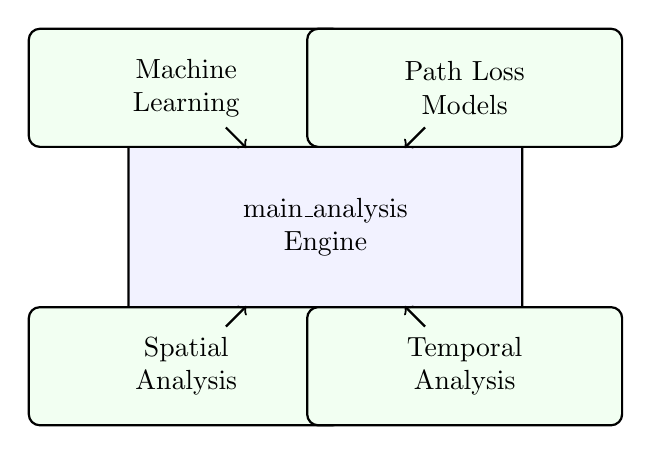
\begin{tikzpicture}[
    node distance=2.5cm,
    class/.style={rectangle, draw=black, thick, minimum width=5cm, minimum height=2.5cm, align=center, fill=blue!5, rounded corners=4pt},
    data/.style={rectangle, draw=black, thick, minimum width=4cm, minimum height=1.5cm, align=center, fill=green!5, rounded corners=4pt},
    arrow/.style={->, thick, black}
]
\node[class] (main) {main\_analysis\\Engine};
\node[data, below left of=main] (spatial) {Spatial\\Analysis};
\node[data, below right of=main] (temporal) {Temporal\\Analysis};
\node[data, above left of=main] (ml) {Machine\\Learning};
\node[data, above right of=main] (models) {Path Loss\\Models};

\draw[arrow] (main) -- (spatial);
\draw[arrow] (main) -- (temporal);
\draw[arrow] (main) -- (ml);
\draw[arrow] (main) -- (models);
\end{tikzpicture}
\caption{Main Analysis Engine integration architecture}
\label{fig:main_analysis_architecture}
\end{figure}

\textbf{Integration with Analysis Scripts:}
The main analysis provides the foundational framework that the Spatial Analysis and the temporal scripts build upon.




\subsection{Spatial Methods:}
The main analysis script implements several standardized analysis methods that are utilized by spatial analysis script:

\textbf{analyze\_coverage\_gaps():}
This method identifies areas along motorways where mobile network coverage is poor or non-existent. It analyzes each coverage point and calculates the percentage of locations with adequate signal strength versus those with poor coverage. The method creates a detailed map of coverage gaps, helping identify where network infrastructure improvements are most needed.

\begin{figure}[H]
   \centering
   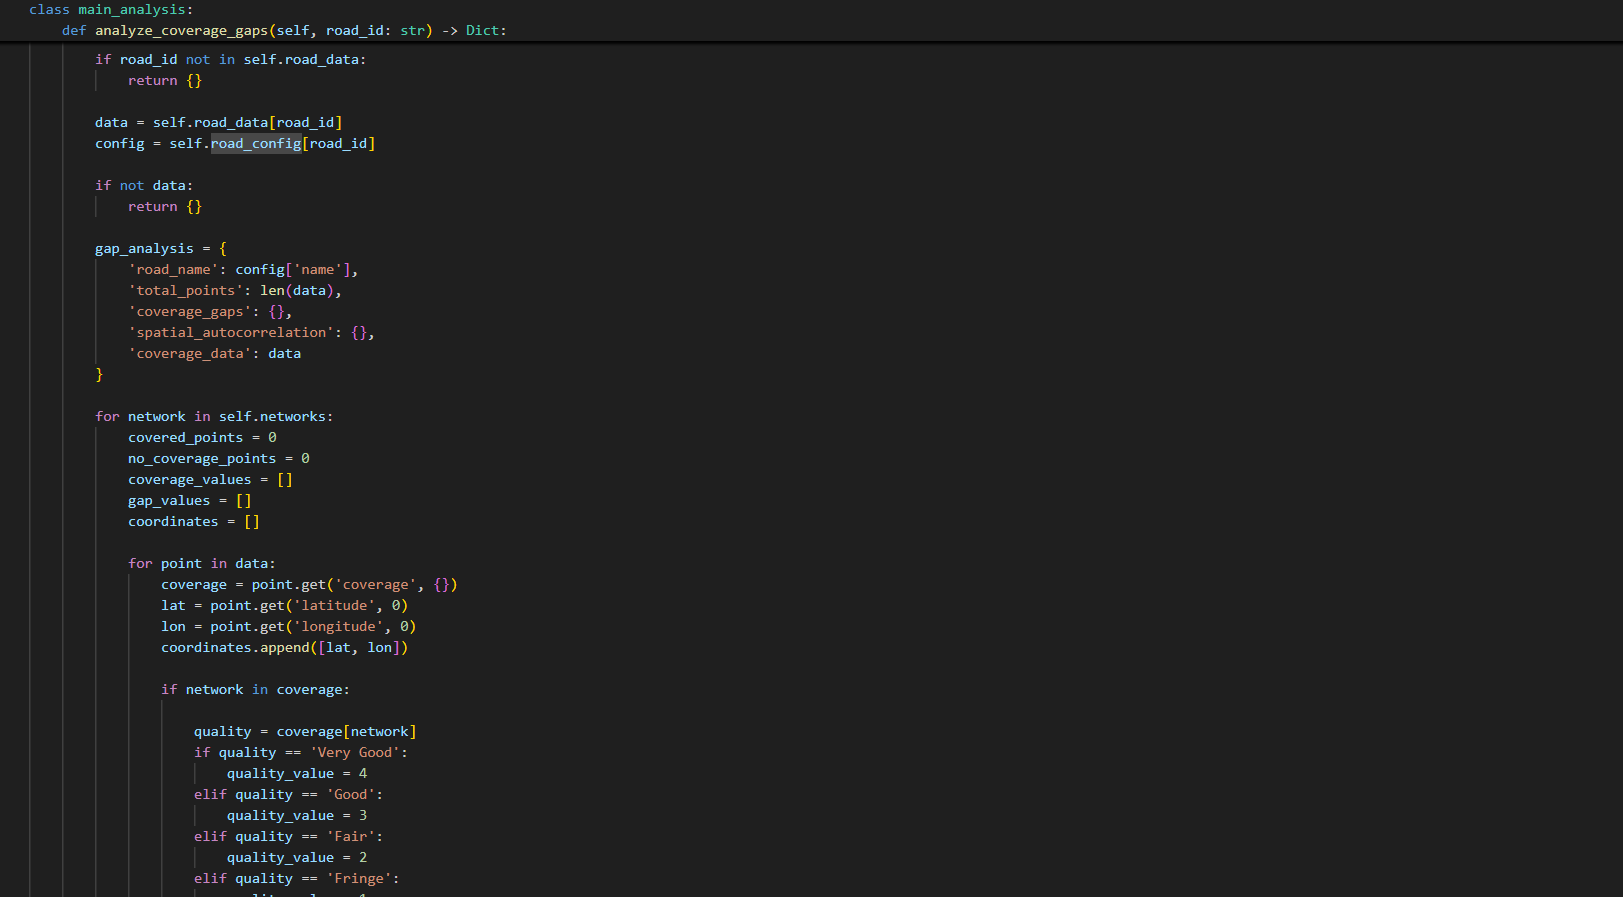
\includegraphics[width=0.8\textwidth]{Images/analyze_coverage_gap.png}
   \caption{Implementation of coverage gaps}
   \label{fig:spatial_coverage_gap}
   \end{figure}

\textbf{analyze\_operator\_comparison():}
This method compares the performance between different mobile network operators (Vodafone and Three) along the motorways. It calculates coverage percentages for each operator's 4G and 5G networks, analyzes quality distributions, and determines which operator provides better service in different geographic areas. This helps understand competitive positioning and service quality differences.

\begin{figure}[H]
   \centering
   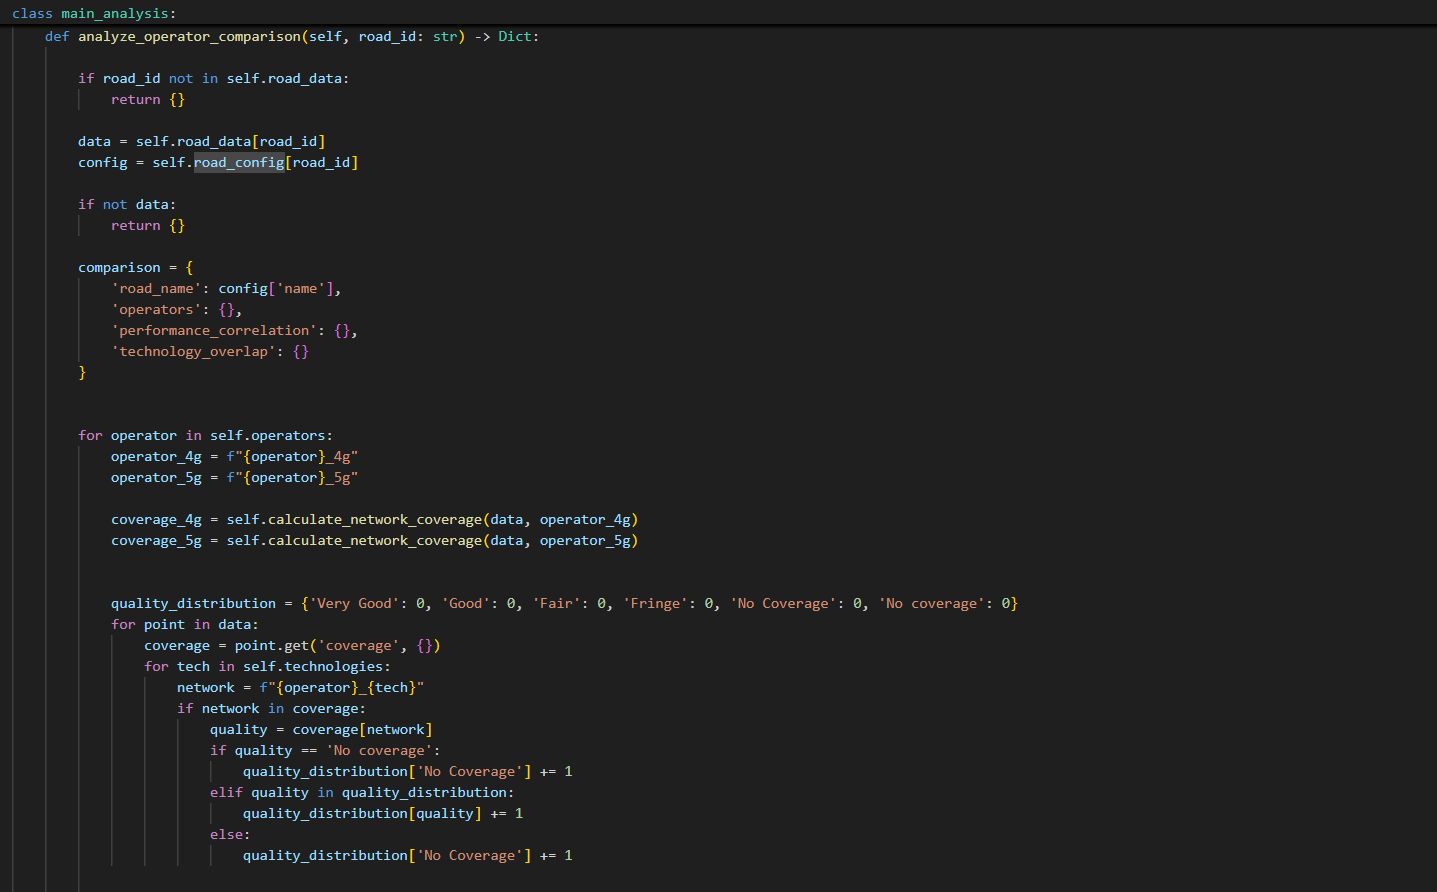
\includegraphics[width=0.8\textwidth]{Images/analyze_operator_comparison.png}
   \caption{Implementation of operator comparison}
   \label{fig:analyze_operator_comparison}
   \end{figure}

\textbf{analyze\_technology\_distribution():}
This method examines how 4G and 5G technologies are distributed across the motorway corridors. It identifies areas where both technologies overlap, locations where only 5G is available (technology transition points), and calculates the overall evolution ratio from 4G to 5G. This analysis helps understand the current state of network modernization and future deployment priorities.

\begin{figure}[H]
   \centering
   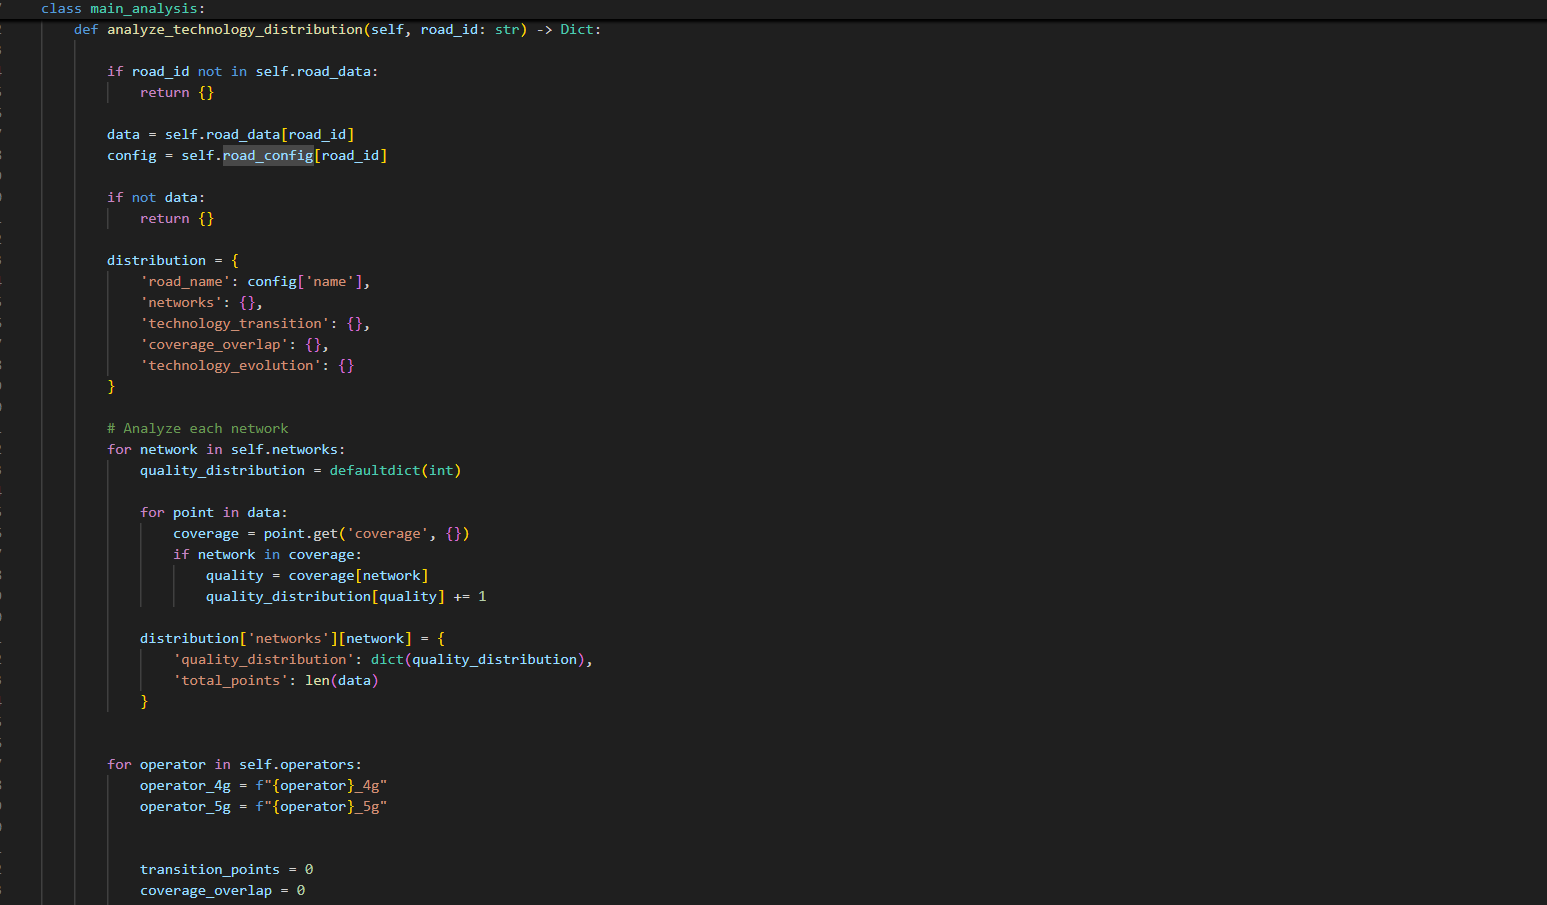
\includegraphics[width=0.8\textwidth]{Images/analyze_technology_distribution.png}
   \caption{Implementation of technology distribution}
   \label{fig:analyze_technology_distribution.}
   \end{figure}
   

\textbf{analyze\_clustering():}
This method uses machine learning algorithms (K-means and DBSCAN) to identify geographic patterns in coverage quality. It groups coverage points into clusters based on their location and signal strength, helping identify areas with similar coverage characteristics. This clustering analysis reveals natural geographic boundaries and coverage zones that may not be immediately obvious from raw data.

\textbf{K-Means Clustering:} Uses $k=5$ clusters (determined by $\min(5, n/10)$ where $n$ is data points) to identify distinct coverage quality zones along motorways.


\textbf{DBSCAN Clustering:} Uses $\epsilon=0.5$ and $\text{min\samples}=5$ to discover natural coverage patterns based on spatial density.

\begin{figure}[H]
   \centering
   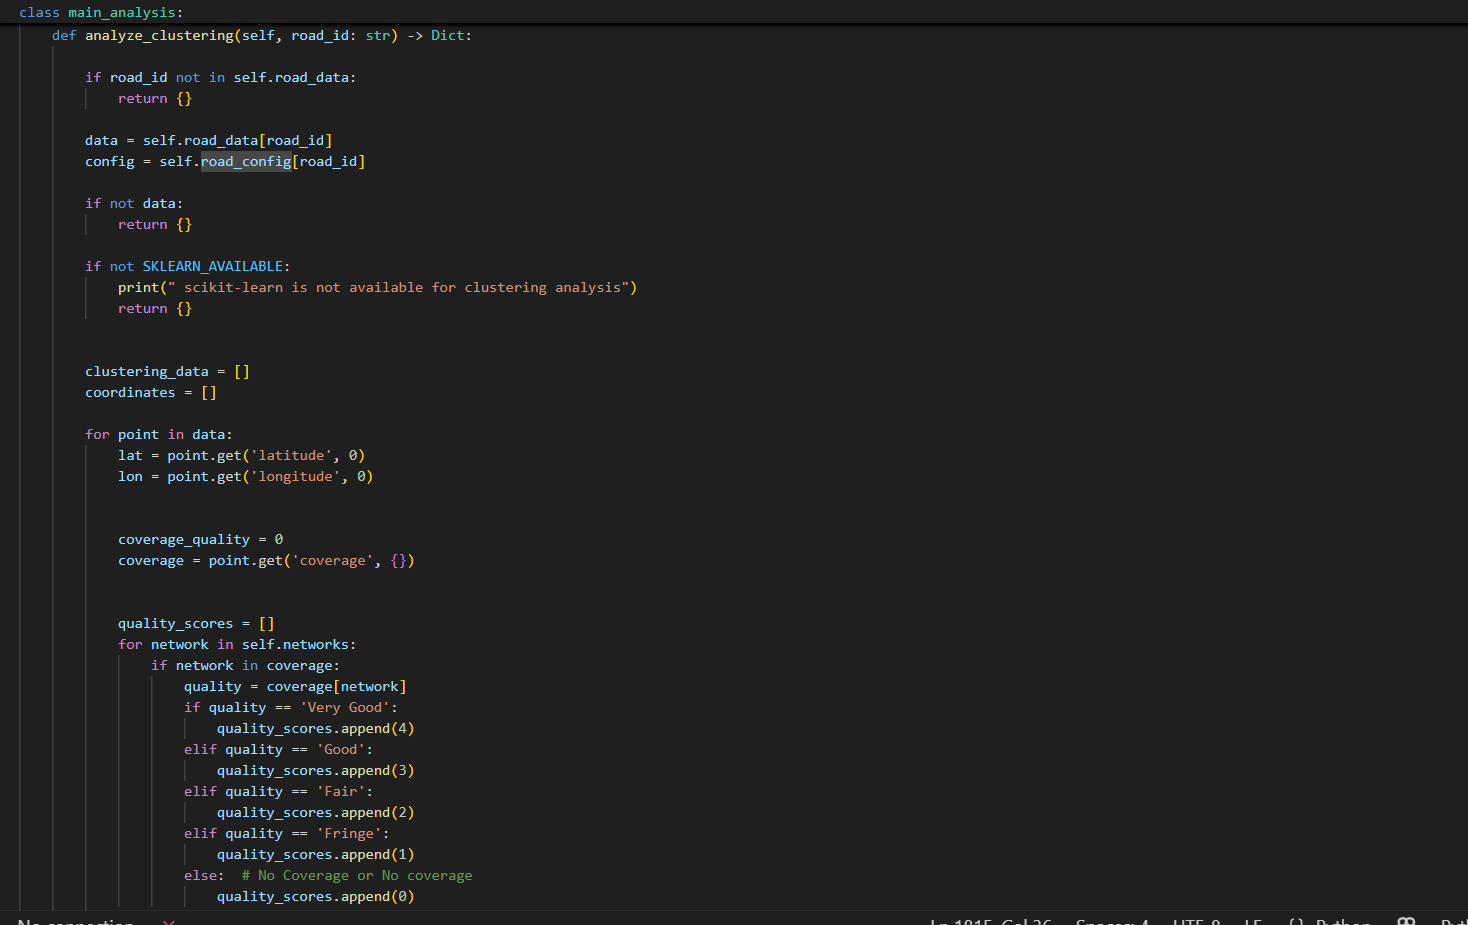
\includegraphics[width=0.8\textwidth]{Images/analyze_clustering.png}
   \caption{Implementation of ML Clustering Algos}
   \label{fig:analyze_clustering}
   \end{figure}

   

\textbf{analyze\_backup\_coverage():}
This method evaluates network redundancy by checking if poor coverage from one network is compensated by good coverage from another network or technology. It calculates overlap percentages between operators and technologies, identifying areas where users have multiple network options versus locations with limited connectivity choices. This analysis is crucial for understanding network reliability and user experience.

\begin{figure}[H]
   \centering
   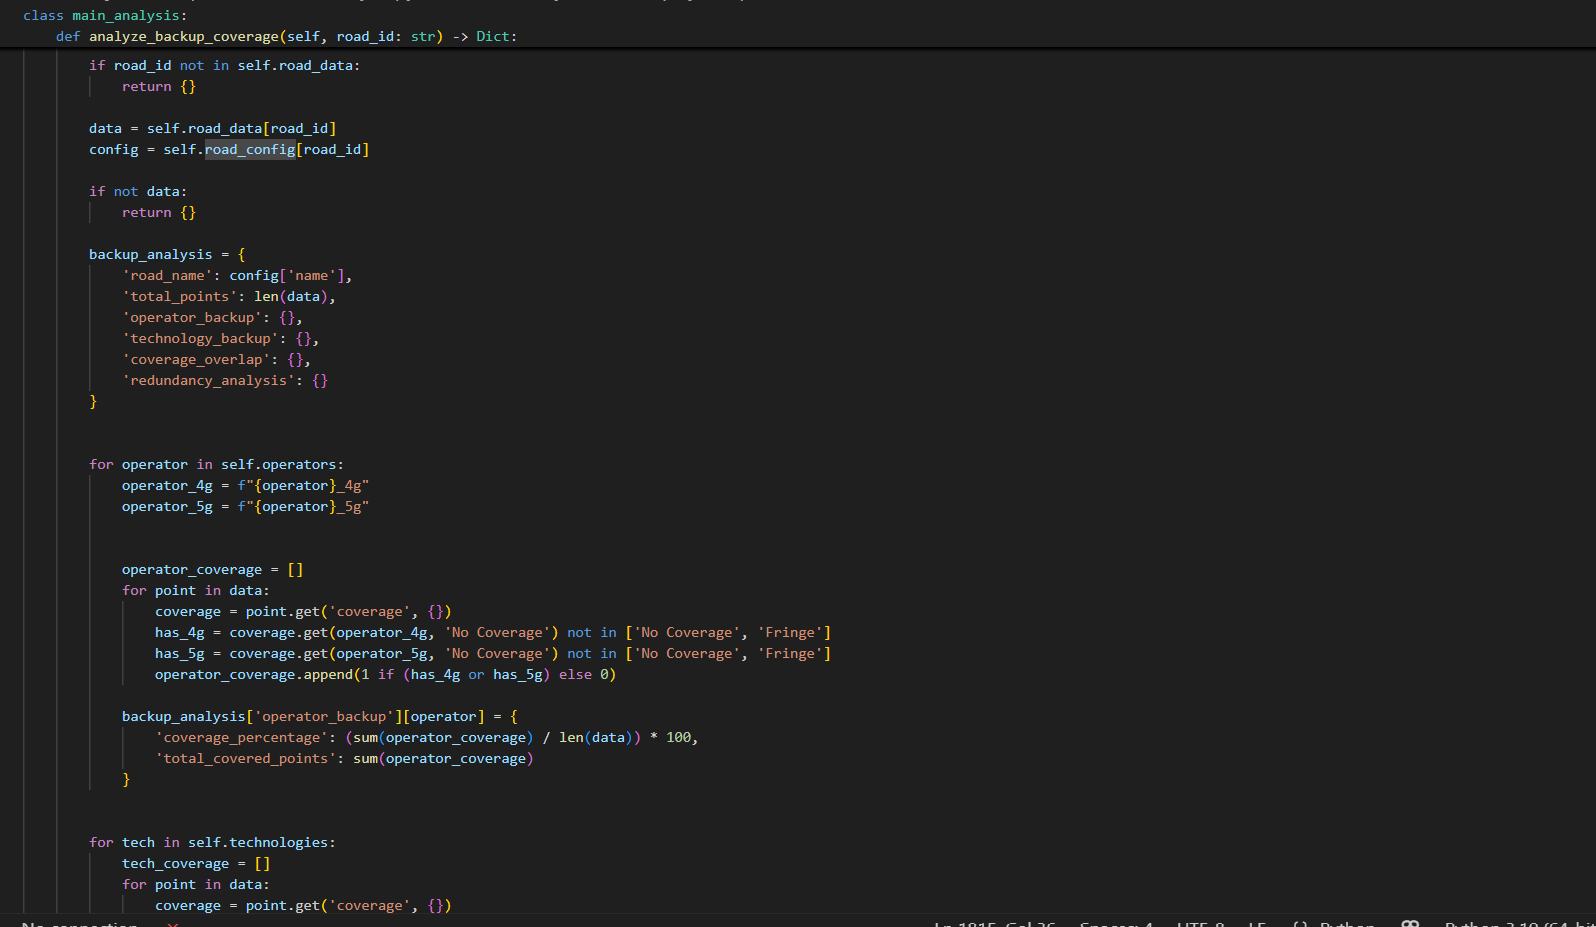
\includegraphics[width=0.8\textwidth]{Images/analyze_backup_coverage.png}
   \caption{Implementation of backup coverage method}
   \label{fig:analyze_backup_coverage}
   \end{figure}
   

\textbf{analyze\_model\_comparison():}
This method compares theoretical path loss model predictions with real-world coverage measurements. It calculates accuracy metrics like Root Mean Square Error (RMSE) and Mean Absolute Error (MAE) to validate how well the mathematical models predict actual coverage. This validation ensures that the theoretical models are reliable for future network planning and capacity assessment.

\begin{figure}[H]
   \centering
   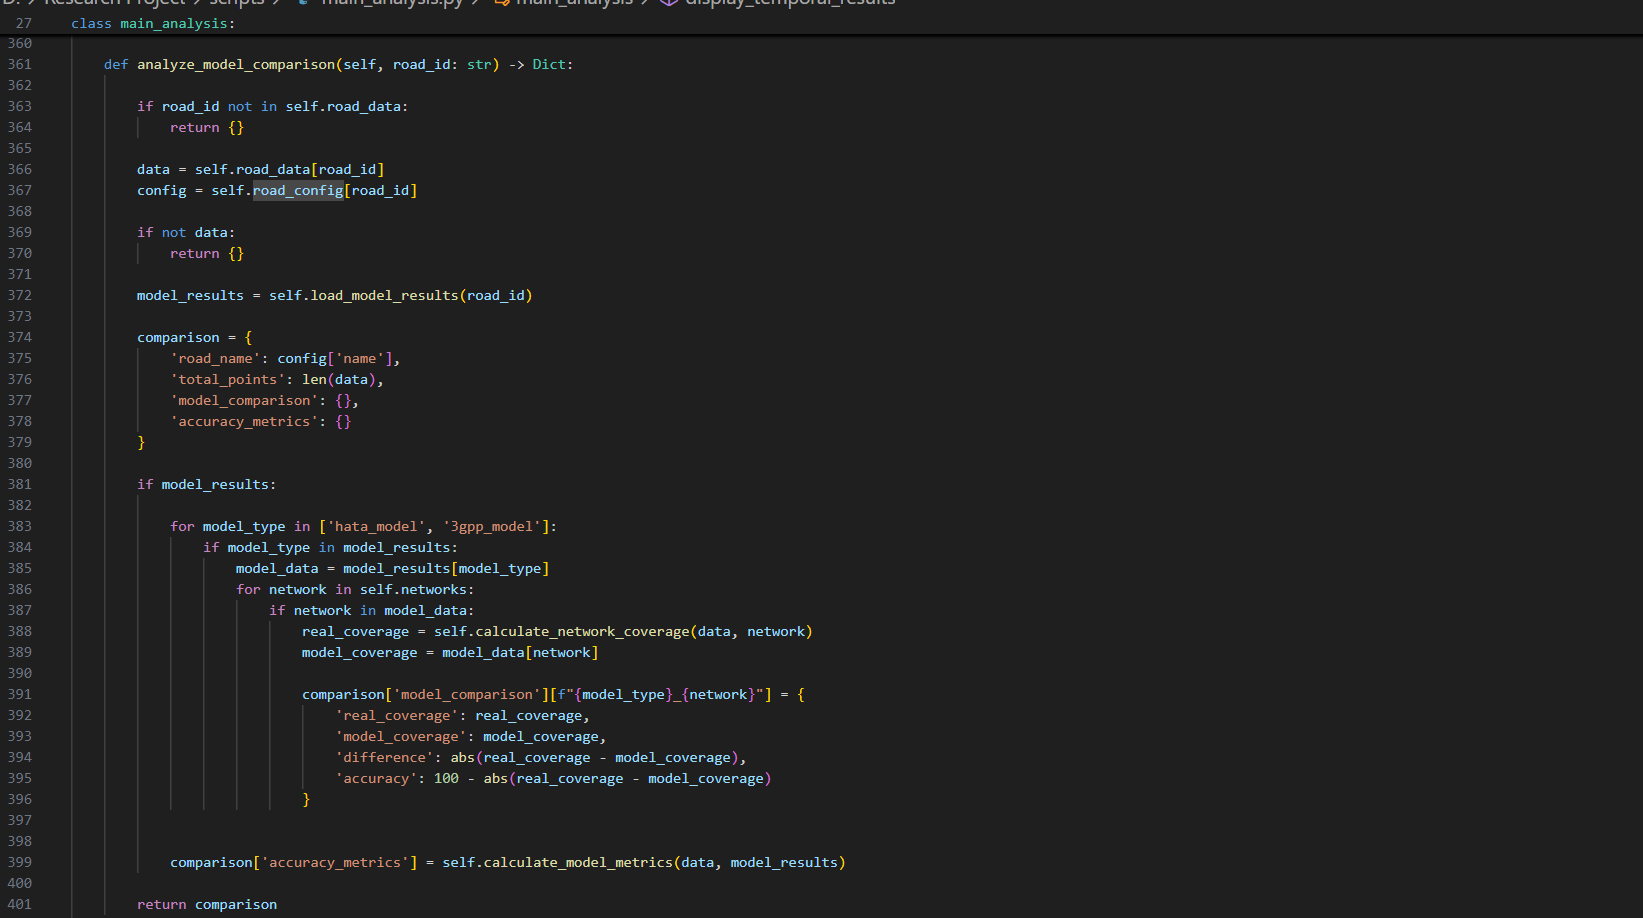
\includegraphics[width=0.8\textwidth]{Images/analyze_model_comparison.png}
   \caption{Implementation of model comparison}
   \label{fig:analyze_model_comparison}
   \end{figure}


\subsection{Temporal Methods:}
The main analysis script implements several standardized temporal analysis methods that are utilized by temporal analysis scripts:

\textbf{analyze\_traffic\_patterns():}
This method analyzes hourly traffic patterns along motorways using TII traffic data. It processes traffic volume data from multiple monitoring sites and calculates hourly distributions, identifying peak traffic periods and traffic flow patterns throughout the day. The method provides comprehensive temporal analysis of traffic behavior, helping understand when network demand is highest and capacity planning requirements.

\begin{figure}[H]
   \centering
   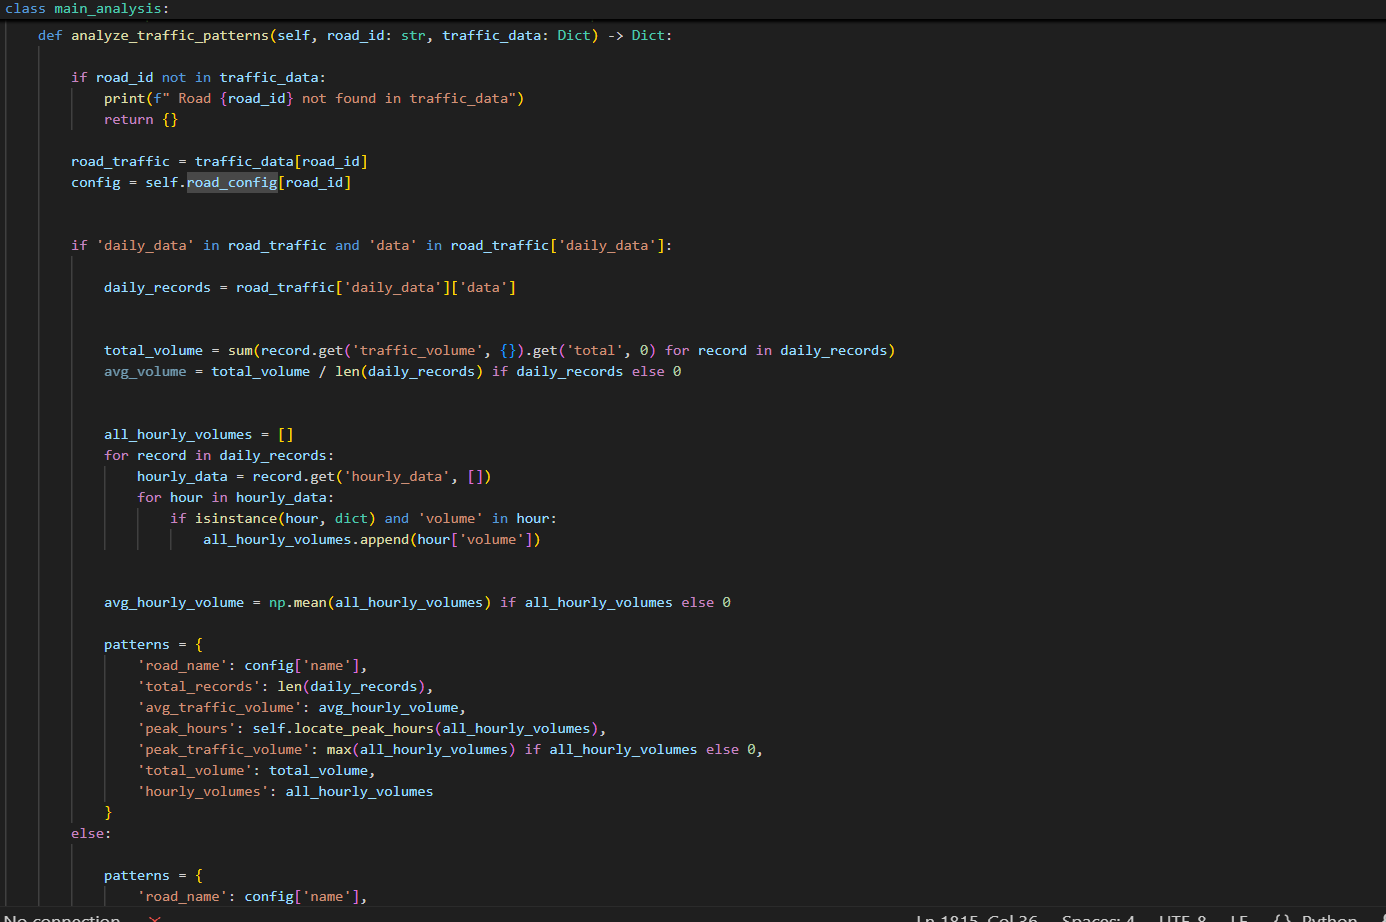
\includegraphics[width=0.8\textwidth]{Images/analyze_traffic_patterns.png}
   \caption{Implementation of traffic pattern analysis}
   \label{fig:temporal_traffic_patterns}
\end{figure}

\textbf{analyze\_morning\_evening\_peaks():}
This method identifies and analyzes morning and evening peak traffic hours along motorways. It calculates peak traffic volumes for morning hours (6-9 AM) and evening hours (4-7 PM), determining the busiest periods when network capacity is most critical. The method provides detailed peak hour analysis, including volume statistics and timing information essential for network capacity planning and infrastructure optimization.

\begin{figure}[H]
   \centering
   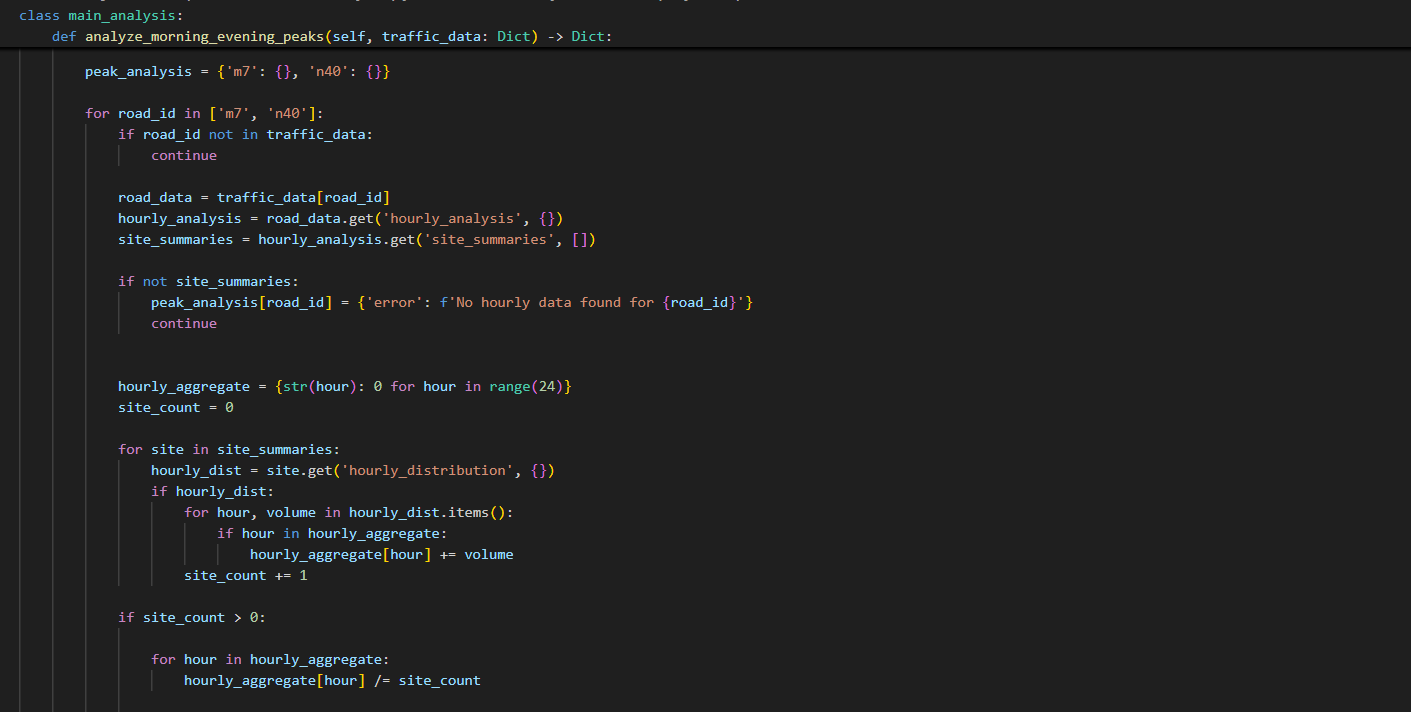
\includegraphics[width=0.8\textwidth]{Images/analyze_peak_hours.png}
   \caption{Implementation of peak hour analysis}
   \label{fig:temporal_peak_hours}
\end{figure}

\textbf{analyze\_multiple\_peak\_hours():}
This method performs comprehensive analysis of multiple peak hours across different monitoring sites. It identifies the most common peak hours across all sites, calculates peak hour distributions, and determines the top volume hours for each motorway. This analysis helps understand traffic patterns across different geographic segments and provides insights for targeted network capacity planning.

\begin{figure}[H]
   \centering
   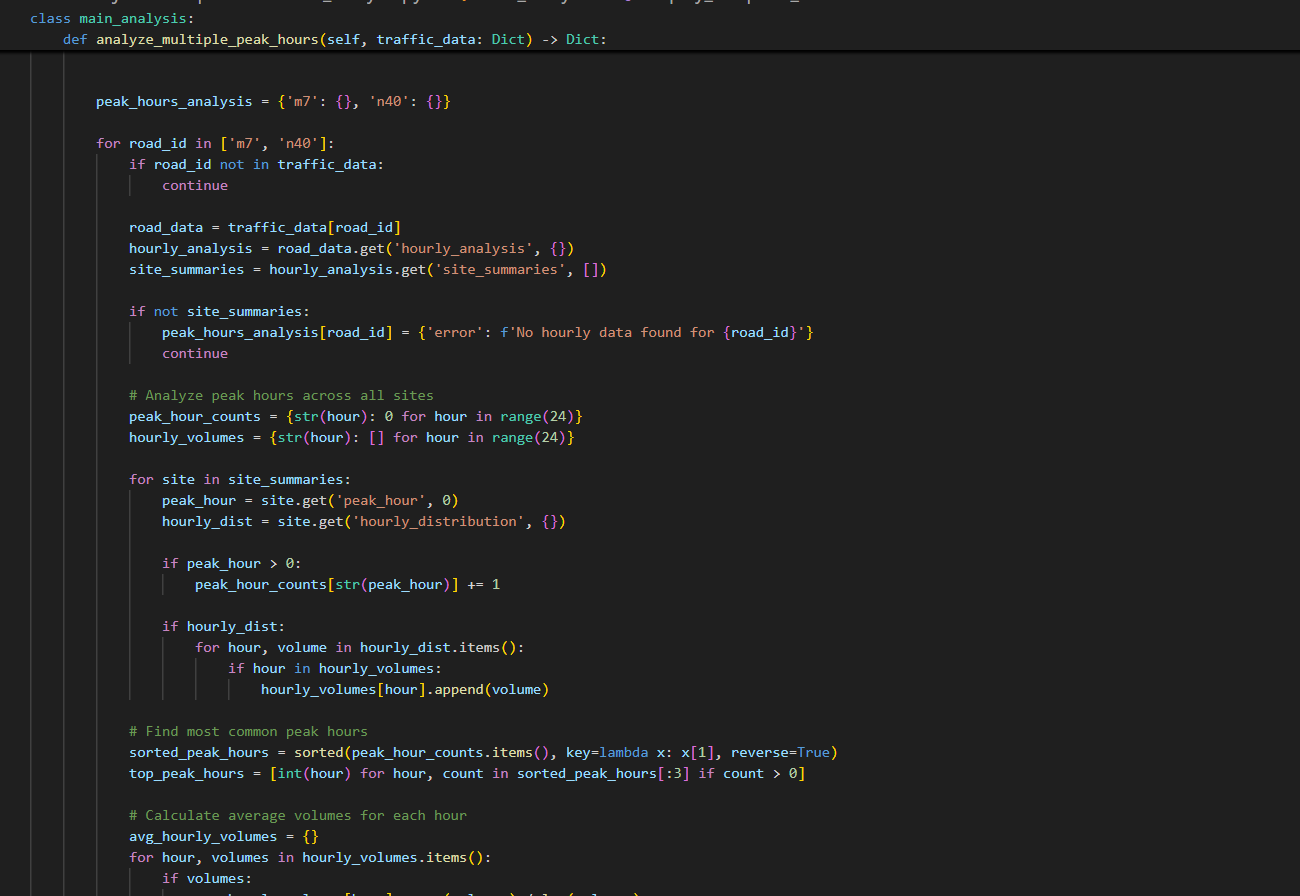
\includegraphics[width=0.8\textwidth]{Images/analyze_multiple_peaks.png}
   \caption{Implementation of multiple peak hour analysis}
   \label{fig:temporal_multiple_peaks}
\end{figure}

\textbf{analyze\_weekday\_weekend\_patterns():}
This method compares traffic patterns between weekdays and weekends using TII weekly data. It calculates average traffic volumes for workdays versus weekend days, determines weekday/weekend ratios, and identifies peak hours for each day type. This analysis is crucial for understanding commuter versus leisure traffic patterns and their implications for network capacity planning.

\begin{figure}[H]
   \centering
   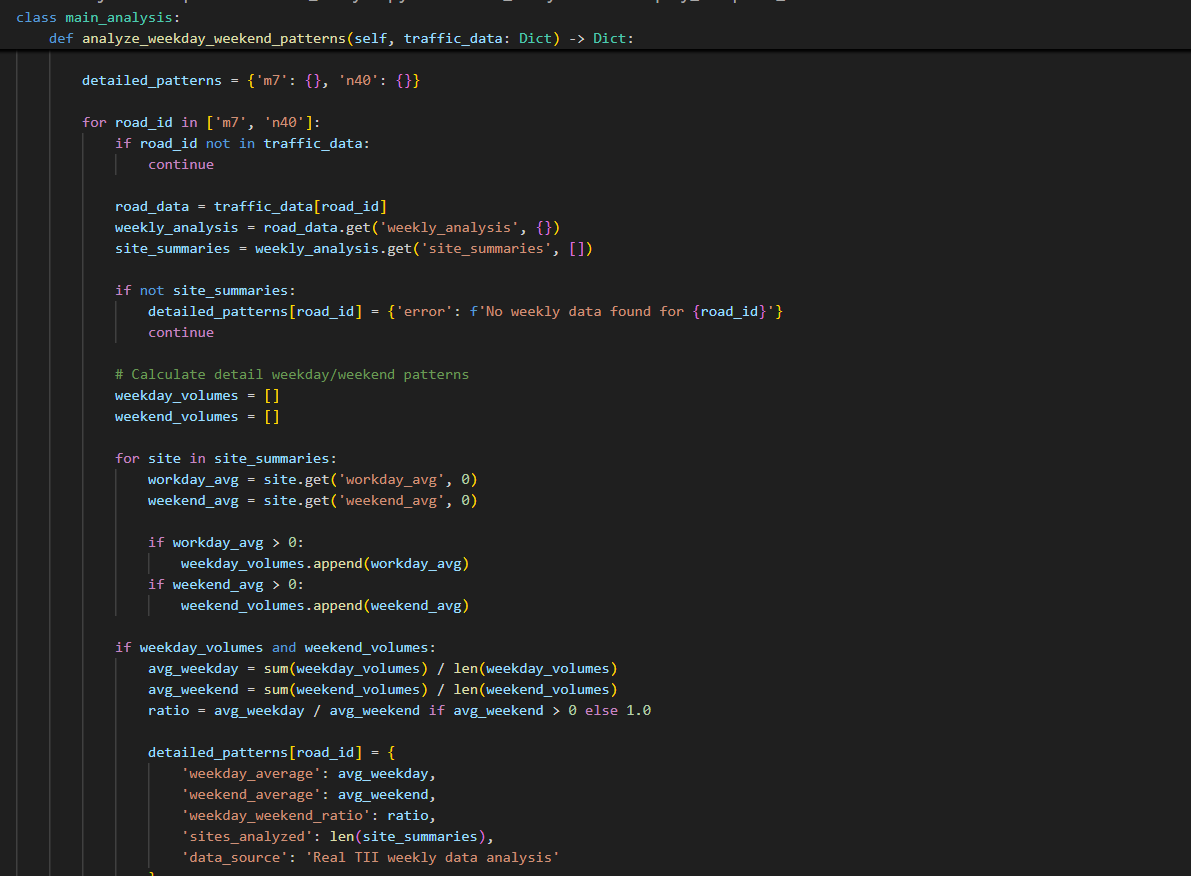
\includegraphics[width=0.8\textwidth]{Images/analyze_weekday_weekend.png}
   \caption{Implementation of weekday/weekend pattern analysis}
   \label{fig:temporal_weekday_weekend}
\end{figure}

\textbf{process\_seasonal\_analysis():}
This method analyzes seasonal traffic patterns across different time periods throughout the year. It categorizes traffic data by seasons (summer, autumn, winter, spring), calculates seasonal statistics, and identifies seasonal traffic patterns. The method provides insights into how traffic volumes vary throughout the year, enabling long-term capacity planning and seasonal network optimization strategies.

\begin{figure}[H]
   \centering
   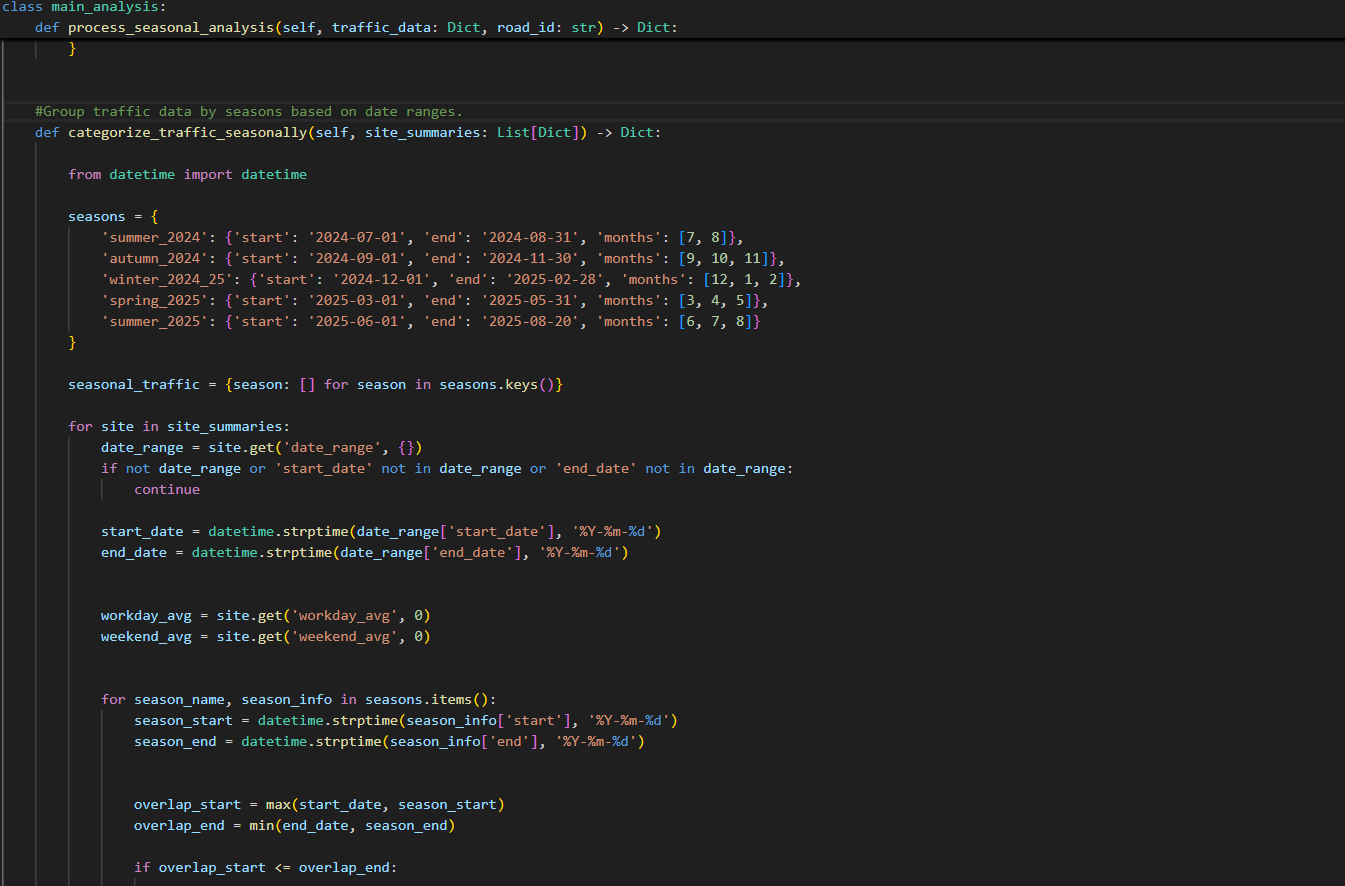
\includegraphics[width=0.8\textwidth]{Images/process_seasonal_analysis.png}
   \caption{Implementation of seasonal analysis}
   \label{fig:temporal_seasonal_analysis}
\end{figure}


\section{Spatial and Temporal Analysis Scripts}

\subsection{Spatial Analysis Script Implementation}
The Spatial Analysis script (`spatial\_analysis.py`) implements comprehensive geographic analysis of mobile network coverage along Irish motorways using the main analysis engine. This script serves as the primary spatial analysis interface, providing detailed coverage assessment and geographic pattern recognition capabilities.

\textbf{Technical Implementation:} The script utilizes the main analysis engine to perform comprehensive spatial analysis without code duplication. The implementation includes robust result display mechanisms, comprehensive data visualization, and standardized output formatting to ensure consistent analysis presentation across different road networks.

\textbf{Analysis Workflow:}
\begin{enumerate}
\item Initialize spatial analyzer with main analysis engine integration
\item Execute complete spatial analysis for both M7 and N40 motorways
\item Display comprehensive results including network coverage, operator comparison, and technology distribution
\item Generate clustering analysis and backup coverage assessment
\item Save detailed results and summary reports for further analysis
\end{enumerate}

\textbf{Core Analysis Components:}
\begin{itemize}
\item \textbf{Network Coverage Analysis:} Comprehensive coverage assessment across all networks and operators
\item \textbf{Provider Comparison:} Detailed comparison between Vodafone and Three network performance
\item \textbf{Technology Distribution:} Analysis of 4G and 5G technology availability and overlap
\item \textbf{Clustering Analysis:} Machine learning-based geographic pattern recognition
\item \textbf{Backup Coverage Assessment:} Network redundancy and reliability analysis
\end{itemize}

\textbf{Output and Data Structure:} The script generates comprehensive spatial analysis results including:
\begin{itemize}
\item Detailed coverage statistics for each network and operator
\item Geographic clustering patterns and coverage zones
\item Technology transition analysis and evolution metrics
\item Network complementarity and redundancy assessment
\item Professional summary reports and visualization data
\end{itemize}

\begin{figure}[H]
\centering
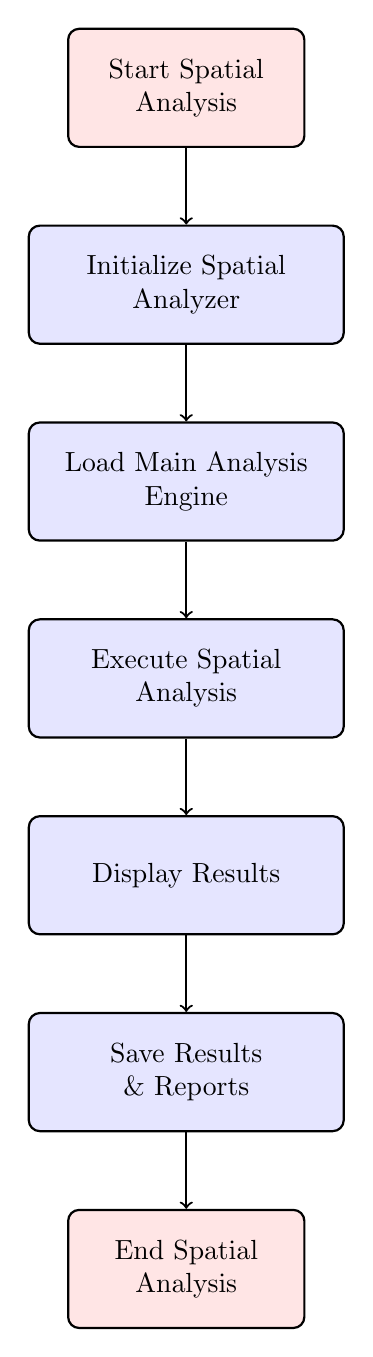
\begin{tikzpicture}[
    node distance=2.5cm,
    startstop/.style={rectangle, draw=black, thick, minimum width=3cm, minimum height=1.5cm, align=center, fill=red!10, rounded corners=4pt},
    process/.style={rectangle, draw=black, thick, minimum width=4cm, minimum height=1.5cm, align=center, fill=blue!10, rounded corners=4pt},
    decision/.style={diamond, draw=black, thick, minimum width=3cm, minimum height=2cm, align=center, fill=green!10},
    arrow/.style={->, thick, black}
]
\node[startstop] (start) {Start Spatial\\Analysis};
\node[process, below of=start] (init) {Initialize Spatial\\Analyzer};
\node[process, below of=init] (main) {Load Main Analysis\\Engine};
\node[process, below of=main] (analyze) {Execute Spatial\\Analysis};
\node[process, below of=analyze] (display) {Display Results};
\node[process, below of=display] (save) {Save Results\\\& Reports};
\node[startstop, below of=save] (end) {End Spatial\\Analysis};

\draw[arrow] (start) -- (init);
\draw[arrow] (init) -- (main);
\draw[arrow] (main) -- (analyze);
\draw[arrow] (analyze) -- (display);
\draw[arrow] (display) -- (save);
\draw[arrow] (save) -- (end);
\end{tikzpicture}
\caption{Spatial Analysis Script workflow}
\label{fig:spatial_analysis_flow}
\end{figure}

\subsection{Temporal Analysis Script Implementation}
The Temporal Analysis script (`temporal\_analysis.py`) implements comprehensive time-based analysis of traffic patterns and network capacity requirements along Irish motorways. This script serves as the primary temporal analysis interface, providing detailed traffic pattern analysis and capacity planning insights.

\textbf{Technical Implementation:} The script utilizes the main analysis engine to perform comprehensive temporal analysis without code duplication. The implementation includes robust data processing mechanisms, comprehensive result formatting, and standardized output generation to ensure consistent temporal analysis presentation.

\textbf{Analysis Workflow:}
\begin{enumerate}
\item Initialize temporal analyzer with main analysis engine integration
\item Execute comprehensive temporal analysis using TII traffic data
\item Process traffic patterns, peak hours, and seasonal variations
\item Generate capacity planning assessments and future scenario modeling
\item Save detailed results and summary reports for further analysis
\end{enumerate}

\textbf{Core Analysis Components:}
\begin{itemize}
\item \textbf{Traffic Pattern Analysis:} Hourly, daily, and seasonal traffic pattern identification
\item \textbf{Peak Hour Analysis:} Statistical identification of peak traffic periods and network stress points
\item \textbf{Weekday vs Weekend Analysis:} Comparative analysis of commuter versus leisure traffic patterns
\item \textbf{Seasonal Analysis:} Long-term traffic trend analysis with seasonal factor calculations
\item \textbf{Capacity Planning:} Current and future network capacity assessment based on traffic projections
\end{itemize}

\textbf{Output and Data Structure:} The script generates comprehensive temporal analysis results including:
\begin{itemize}
\item Detailed traffic pattern statistics and peak hour identification
\item Weekday/weekend traffic pattern comparisons and ratios
\item Seasonal traffic variations and trend analysis
\item Network capacity assessments for different vehicle scenarios
\item Professional summary reports and temporal visualization data
\end{itemize}

\begin{figure}[H]
\centering
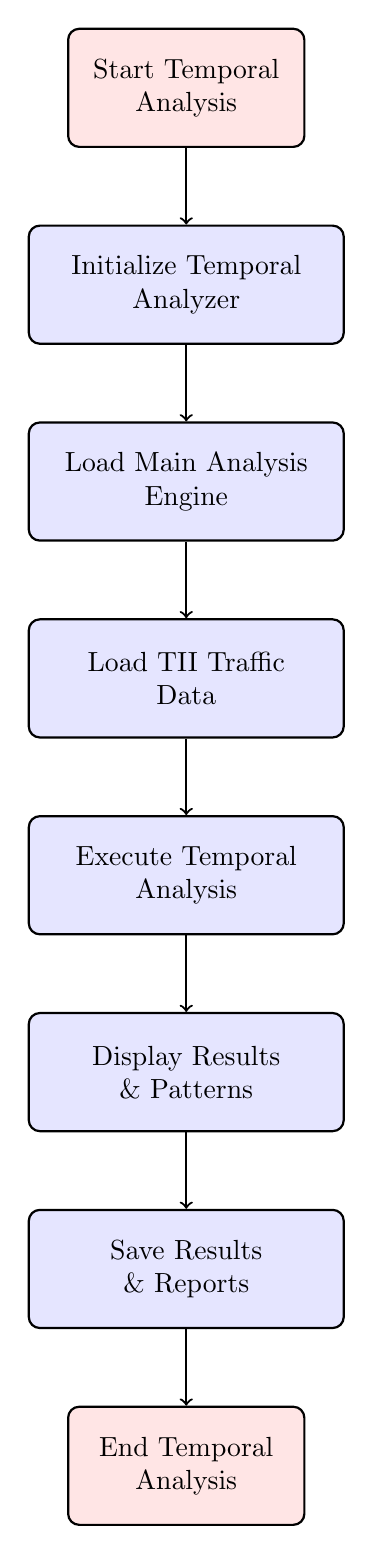
\begin{tikzpicture}[
    node distance=2.5cm,
    startstop/.style={rectangle, draw=black, thick, minimum width=3cm, minimum height=1.5cm, align=center, fill=red!10, rounded corners=4pt},
    process/.style={rectangle, draw=black, thick, minimum width=4cm, minimum height=1.5cm, align=center, fill=blue!10, rounded corners=4pt},
    decision/.style={diamond, draw=black, thick, minimum width=3cm, minimum height=2cm, align=center, fill=green!10},
    arrow/.style={->, thick, black}
]
\node[startstop] (start) {Start Temporal\\Analysis};
\node[process, below of=start] (init) {Initialize Temporal\\Analyzer};
\node[process, below of=init] (main) {Load Main Analysis\\Engine};
\node[process, below of=main] (traffic) {Load TII Traffic\\Data};
\node[process, below of=traffic] (analyze) {Execute Temporal\\Analysis};
\node[process, below of=analyze] (display) {Display Results\\\& Patterns};
\node[process, below of=display] (save) {Save Results\\\& Reports};
\node[startstop, below of=save] (end) {End Temporal\\Analysis};

\draw[arrow] (start) -- (init);
\draw[arrow] (init) -- (main);
\draw[arrow] (main) -- (traffic);
\draw[arrow] (traffic) -- (analyze);
\draw[arrow] (analyze) -- (display);
\draw[arrow] (display) -- (save);
\draw[arrow] (save) -- (end);
\end{tikzpicture}
\caption{Temporal Analysis Script workflow}
\label{fig:temporal_analysis_flow}
\end{figure}

\subsection{Integration with Main Analysis Engine}
Both spatial and temporal analysis scripts demonstrate the modular architecture of the analysis framework, utilizing the main analysis engine to provide specialized analysis capabilities while maintaining code consistency and avoiding duplication. This integration approach ensures:

\begin{itemize}
\item \textbf{Code Reusability:} Common analysis methods are shared through the main analysis engine
\item \textbf{Consistency:} Standardized analysis protocols and output formats across all analysis types
\item \textbf{Maintainability:} Centralized code management reduces maintenance overhead
\item \textbf{Scalability:} Easy extension to additional road networks and analysis types
\item \textbf{Reliability:} Proven analysis methods ensure consistent and accurate results
\end{itemize}

The modular design allows each script to focus on its specialized analysis domain while leveraging the robust foundation provided by the main analysis engine, resulting in efficient, maintainable, and reliable analysis workflows.


\section{Network Capacity Assessment Scenarios}

\subsection{Introduction to Capacity Assessment}
Network capacity assessment is crucial for understanding whether current mobile infrastructure can support projected vehicular traffic demands. This analysis bridges the gap between theoretical coverage models and practical network planning, providing insights into real-world network performance under realistic traffic conditions. By evaluating capacity scenarios, we can assess the adequacy of current infrastructure and identify future upgrade requirements.

\subsection{Network Capacity Assessment Scenarios}
To evaluate whether Irish 4G/5G networks can support typical motorway traffic, we examine two stress test scenarios on the M7 and N40. These routes carry very high flows , for example, the M7 (outer cordon) averaged about 102,250 vehicles/day (6.3\% heavy goods vehicles)\cite{tii_m7_traffic}, and sections of the N40 exceed 80,000 to 100,000 vehicles/day \cite{tii_n40_traffic}.  " Underlying vehicle mix on such roads is mostly private cars (with average occupancy roughly 1.3 to 1.5 persons."\cite{eea_occupancy}) plus a fraction of heavy trucks and buses. We assume about 200 vehicles present in a stretch at once: e.g.\ 180 cars (=270 passengers) and 20 trucks (20 drivers).

\paragraph{Scenario 1: Mixed usage.} In this scenario each vehicle's occupants generate a mix of moderate data (web, email) and some video. Industry data suggest an average smartphone user in Ireland consumes $\sim$18.7 GB per month.\cite{comreg_mobile_usage} , (=0.62 GB per day) under typical usage. Peak-hour usage can be much higher; for example, streaming 1080p video uses 1.5 to 3 GB/hour\cite{roamless_streaming}. For a heavy-traffic calculation we assume each passenger generates on the order of 0.2 GB in one hour (200 MB/h) , a conservative average given the possibility of video. With roughly 290 users in the 200 vehicles, this yields $\approx 58$ GB of data in one hour (around 160 Mb/s sustained). This demand estimate is compatible with moderate streaming activity (0.2 GB/h per user is much less than a full HD stream\cite{roamless_streaming} but several times the off-peak average\cite{comreg_mobile_usage}).

 \paragraph{Scenario 2: All-streaming.} Here we assume 100 cars (one occupant streaming) each concurrently stream high-definition video. Taking $\sim$2.5 GB per car-hour (midpoint of 2–3 GB/h for 1080p\cite{roamless_streaming}), the aggregate load is $\sim$250 GB in one hour, i.e.\ about 0.56 Gb/s. Even more extremely, if each car used 3 GB/h, total demand would reach $\sim$300 GB/h (≈0.67 Gb/s). This represents very high simultaneous throughput for a single cell.

\subsection{Network Capacity Assumptions}
We analyze the capacity of either of the major Irish operators (Vodafone or Three). Both maintain $\sim$2.3 to 2.4 thousand base station sites nationwide\cite{comreg_base_stations}, each with multiple sectors and carriers. Typical LTE (4G) and 5G specifications imply the following per site capabilities: a single 20 MHz LTE carrier can peak at $\sim$100 Mb/s\cite{artizanetworks_lte}. In practice operators aggregate carriers (e.g.\ multiple 20 MHz on 800/1800 MHz bands) and deploy 4 into 4 or 8 into 8 MIMO, so an LTE sector might deliver a few hundred Mb/s under good conditions. Modern 5G adds wide channels (e.g.\ 100 MHz in mid band) and higher MIMO. For instance, a 100 MHz 5G NR carrier with 8 spatial streams can theoretically reach several Gbps (about 4.6 Gb/s peak\cite{devopedia_5g}). In summary, a single well equipped 5G sector could exceed 1 Gb/s under ideal conditions, whereas a single LTE sector may be limited to a few hundred Mb/s. We also note that low band spectrum (700/800 MHz) provides broad coverage, while mid band (3.6 GHz) boosts capacity\cite{comreg_spectrum}.

\subsection{Results and Analysis}
Under the mixed usage Scenario 1 ( - 160 Mb/s aggregate), the demand is within the order of magnitude of a single cell's capacity. A typical base station sector with carrier aggregation (e.g.\ 40 to 60 MHz total) can sustain >100 Mb/s, and two sectors cover different directions. Even if the 290 users were unevenly distributed, the load per cell would be modest (e.g.\ 80 to 100 Mb/s per sector). Thus current 4G/5G coverage along the motorway would likely accommodate this demand with some margin, assuming no other large traffic surge.

In Scenario 2, however, the demand approaches the limits of one sector. About 0.5 to 0.7 Gb/s sustained would be required if all 100 cars streamed simultaneously. A single LTE sector ($\sim$100 Mb/s per 20 MHz) cannot carry this by itself; even with carrier aggregation it would need several carriers (and uplink would be stressed). A 5G sector with 100 MHz could in theory handle it (peak 4 to 5 Gb/s\cite{devopedia_5g}), but that assumes pristine conditions on every channel. In reality, if all 100 cars were in one cell, throughput would be bottlenecked. We can conclude Scenario 2 would likely exceed the practical capacity of a single LTE cell and strain a single 5G cell. (In practice, motorway coverage comes from multiple sites, so traffic would split among cells; but the scenario highlights that very high simultaneous demand may saturate the network.)

\subsection{Future Projections and Improvements}
Looking ahead, connected/autonomous vehicles will further increase demands. ComReg expects that in vehicle infotainment and driver assist services will grow rapidly, while fully autonomous cars (requiring ultra low latency) are a longer term prospect (beyond mid 2020s)\cite{comreg_autonomous}. Still, even today advanced driver aids involve HD mapping and sensor data exchange. Studies (e.g.\ the 5GCroCo project) note that tele operated driving requires very high uplink data rates for video streaming from vehicles\cite{5gcroc_project}. These trends imply that road networks will face multi gigabit loads in the future.

 To do this, infrastructure must be upgraded. For example, Vodafone announced plans to add 150 new 5G sites along Germany's autobahn network by 2026\cite{vodafone_autobahn}. By analogy, Irish motorways would benefit from many additional sites (small cells or macro sites) to densify coverage and capacity. Expanding mid band 5G (e.g.\ 3.6 GHz) and leveraging new low band licenses (e.g.\ 700 MHz) will boost throughput and range. Coordinated planning with transport authorities (as in Germany\cite{vodafone_autobahn}) can locate towers at rest areas or infrastructure. Network optimization features (beamforming, edge computing, network slicing) will also be needed to support vehicle‐critical traffic.

\subsection{Conclusions}
Using Irish data and conservative assumptions, we find current networks can sustain a moderate multi user scenario (Scenario 1) but struggle under an extreme streaming load (Scenario 2). 
The M7/N40 road traffic($\sim10^{5}$~vpd~\cite{tii_m7_traffic}\cite{tii_n40_traffic}) with typical usage likely stays within cell capacities. However, 100 simultaneous HD streams (~0.5 to 0.7 Gb/s) would challenge a single operator's cell bandwidth. In practice, carriers (Vodafone and Three) should therefore continue enhancing network capacity along these routes. Recommendations include deploying more 5G cells along the motorways, adding spectrum bandwidth, and preparing for the heavy uplink and low latency needs of future autonomous vehicles\cite{comreg_autonomous}\cite{5gcroc_project}. With these measures, the network can remain sufficient for growing vehicular demands.

\begin{center}
\fbox{\parbox{0.95\textwidth}{
\textbf{Summary:} This capacity assessment builds upon our spatial and temporal coverage analysis. The coverage gaps identified in our spatial analysis directly impact capacity scenarios, as areas with poor coverage cannot support high-bandwidth applications regardless of theoretical capacity. Similarly, the temporal traffic patterns analyzed influence when capacity constraints are most likely to occur. The capacity scenarios reference broader TII and ComReg studies with larger datasets than our specific analysis, demonstrating the practical application of our theoretical models in real-world network planning.
}}
\end{center}


 \section{Implementation Details}

   \subsection{Software Architecture}
   The analysis was implemented using:
   \begin{itemize}
   \item Python 3.9+ for data processing and analysis
   \item Pandas for data manipulation and statistical analysis
   \item NumPy for numerical computations
   \item Scikit-learn for clustering and machine learning
   \end{itemize}

    \text
   The below figure shows a layered software architecture followed by this research, it is a 5-layer architecture (Top to Bottom)

   \begin{figure}[h]
   \centering
   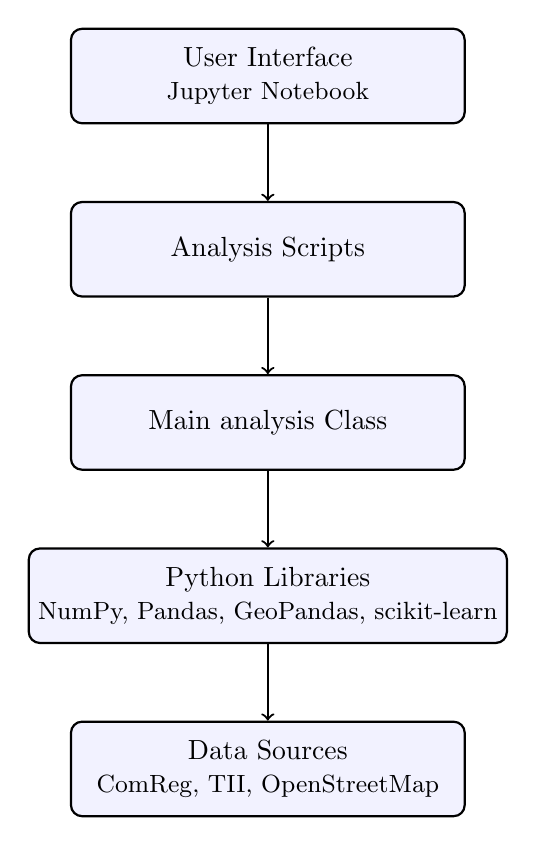
\begin{tikzpicture}[
       node distance=2.2cm,
       box/.style={rectangle, draw=black, thick, minimum width=5cm, minimum height=1.2cm, align=center, fill=blue!5, rounded corners=4pt},
       arrow/.style={->, thick, black}
   ]
   \node[box] (ui) {User Interface\\\small{Jupyter Notebook}};
   \node[box, below of=ui] (Spatial and Temporal) { Analysis Scripts};
   \node[box, below of=Spatial and Temporal] (main) {Main analysis Class};
   \node[box, below of=main] (libs) {Python Libraries\\\small{NumPy, Pandas, GeoPandas, scikit-learn}};
   \node[box, below of=libs] (data) {Data Sources\\\small{ComReg, TII, OpenStreetMap}};

   \draw[arrow] (ui) -- (Spatial and Temporal);
   \draw[arrow] (Spatial and Temporal) -- (main);
   \draw[arrow] (main) -- (libs);
   \draw[arrow] (libs) -- (data);
   \end{tikzpicture}
   \caption{Software architecture}
   \label{fig:software_arch}
   \end{figure}

   
   \subsection{Data Processing Pipeline}
   The data processing pipeline included:
   \begin{itemize}
   \item Data loading and validation from ComReg and TII sources
   \item Geographic coordinate processing and standardization
   \item Coverage quality classification using verified thresholds
   \item Traffic pattern analysis and peak hour identification
   \item Statistical computation and model validation
   \item Results generation and comprehensive reporting
   \end{itemize}


   \chapter{Results}

\section{Spatial Analysis Results}

\subsection{Network Coverage Analysis}

The spatial analysis examined 12,238 coverage points across both motorways, providing comprehensive insights into mobile network performance along Irish motorways.

\begin{table}[h]
\centering
\caption{Network Coverage Performance Comparison}
\label{tab:network_coverage}
\begin{tabular}{|l|c|c|c|c|}
\hline
\textbf{Network} & \textbf{M7 4G (\%)} & \textbf{M7 5G (\%)} & \textbf{N40 4G (\%)} & \textbf{N40 5G (\%)} \\
\hline
Vodafone & 98.2 & 68.6 & 97.3 & 97.3 \\
\hline
Three & 99.0 & 96.2 & 97.3 & 97.3 \\
\hline
\textbf{Average} & \textbf{98.6} & \textbf{82.4} & \textbf{97.3} & \textbf{97.3} \\
\hline
\end{tabular}
\end{table}

\textbf{Key Findings:}
\begin{itemize}
\item M7 Dublin-Limerick shows significant 5G coverage disparity between operators (68.6\% vs 96.2\%)
\item N40 Cork Ring Road demonstrates uniform coverage across all networks (97.3\%)
\item Overall coverage rate of 98.9\% indicates excellent network infrastructure
\item M7 has 1,731 no-signal areas compared to N40's 120 no-signal areas
\end{itemize}

\textbf{Conclusions:} The results reveal that N40, as an urban motorway, benefits from superior network infrastructure with consistent coverage across all operators and technologies. M7, being primarily rural, shows operator-specific 5G deployment strategies, with Three achieving significantly better 5G coverage than Vodafone. This suggests that rural motorways require targeted infrastructure investment to achieve urban-level coverage standards.

\subsection{Technology Distribution Analysis}

\begin{table}[h]
\centering
\caption{4G vs 5G Technology Distribution}
\label{tab:technology_distribution}
\begin{tabular}{|l|c|c|c|}
\hline
\textbf{Metric} & \textbf{M7 } & \textbf{N40} & \textbf{Implications} \\
\hline
4G Average & 98.6\% & 97.3\% & M7 has better 4G coverage \\
\hline
5G Average & 82.4\% & 97.3\% & N40 has superior 5G deployment \\
\hline
4G-5G Overlap & 74.3\% & 97.3\% & N40 has near-universal dual coverage \\
\hline
4G-only Areas & 24.3\% & 0.0\% & M7 has significant 4G-only zones \\
\hline
5G-only Areas & 1.4\% & 2.7\% & Limited 5G-only coverage on both \\
\hline
\end{tabular}
\end{table}

\textbf{Conclusions:} The technology distribution analysis demonstrates that N40 has achieved near-complete 5G deployment with 97.3\% coverage, while M7 lags significantly at 82.4\%. This indicates that urban motorways have benefited from more aggressive 5G infrastructure investment. The high 4G-5G overlap on N40 (97.3\%) suggests excellent network redundancy, while M7's 24.3\% 4G-only areas represent opportunities for future 5G expansion.

\subsection{Clustering Analysis}

\begin{table}[h]
\centering
\caption{Machine Learning Clustering Results}
\label{tab:clustering_results}
\begin{tabular}{|l|c|c|c|c|}
\hline
\textbf{Road} & \textbf{Algorithm} & \textbf{Clusters} & \textbf{Quality Score} & \textbf{Pattern Description} \\
\hline
M7  & K-Means & 5 & 0.714 & High-quality geographic clustering \\
\hline
M7  & DBSCAN & 1 & 0.000 & Single cluster with noise analysis \\
\hline
N40 & K-Means & 5 & 0.812 & Excellent clustering quality \\
\hline
N40 & DBSCAN & 2 & 0.894 & Density-based clustering \\
\hline
\end{tabular}
\end{table}

\textbf{Clustering Insights:}
\begin{itemize}
\item M7 K-Means identified 5 distinct coverage zones with varying quality levels
\item N40 achieved superior clustering quality (0.812 vs 0.714) indicating more consistent coverage patterns
\item DBSCAN results show N40 has better-defined coverage boundaries than M7
\item Coverage quality ranges from "Fair" (2.03) to "Very Good" (3.91) on M7
\item N40 shows predominantly "Very Good" coverage (3.71 average)
\end{itemize}

\textbf{Conclusions:} The clustering analysis reveals that N40 has more homogeneous coverage patterns, reflected in its higher clustering quality scores. M7's lower clustering quality indicates more variable coverage characteristics, likely due to its rural nature and varying terrain. The identification of distinct coverage zones provides valuable insights for targeted network optimization and infrastructure planning.

\subsection{Backup Coverage Analysis}

\begin{table}[H]
\centering
\caption{Network Redundancy and Backup Coverage}
\label{tab:backup_coverage}
\begin{tabular}{|l|c|c|c|}
\hline
\textbf{Metric} & \textbf{M7} & \textbf{N40} & \textbf{Significance} \\
\hline
Vodafone Backup & 98.5\% & 100.0\% & N40 has perfect Vodafone coverage \\
\hline
Three Backup & 99.6\% & 100.0\% & Both roads have excellent Three coverage \\
\hline
4G Backup & 99.6\% & 100.0\% & Universal 4G coverage on both roads \\
\hline
5G Backup & 98.4\% & 100.0\% & N40 has perfect 5G backup coverage \\
\hline
All Operators Coverage & 98.4\% & 100.0\% & N40 has complete redundancy \\
\hline
No Coverage Areas & 0.3\% & 0.0\% & Minimal coverage gaps on both roads \\
\hline
\end{tabular}
\end{table}

\textbf{Conclusions:} The backup coverage analysis demonstrates that N40 achieves perfect network redundancy with 100\% coverage from all operators and technologies. M7, while maintaining excellent overall coverage (98.4\% all-operators coverage), has small coverage gaps (0.3\%) that represent critical areas for infrastructure improvement. The results indicate that urban motorways benefit from superior network redundancy compared to rural routes.

\section{Temporal Analysis Results}

\subsection{Traffic Pattern Analysis}

The temporal analysis examined traffic patterns across 29 monitoring sites over a comprehensive period, revealing significant insights into motorway usage patterns.

\begin{table}[H]
\centering
\caption{Traffic Volume Analysis Summary}
\label{tab:traffic_analysis}
\begin{tabular}{|l|c|c|c|}
\hline
\textbf{Metric} & \textbf{M7} & \textbf{N40} & \textbf{Total} \\
\hline
Average Hourly Traffic & 1,496 v/hr & 2,877 v/hr & 4,373 vehicles/hour \\
\hline
Daily Traffic & 35,907 v/day & 69,050 v/day & 104,957 vehicles/day \\
\hline
Peak Hourly Traffic & 2,766 v/hr & 5,628 v/hr & 8,394 vehicles/hour \\
\hline
Total Volume & 718,148 vehicles & 552,397 vehicles & 1,270,545 vehicles \\
\hline
Peak-to-Average Ratio & 1.85 & 1.96 & 1.92 \\
\hline
Monitoring Sites & 21 sites & 8 sites & 29 sites \\
\hline
\end{tabular}
\end{table}

\textbf{Conclusions:} The traffic analysis reveals that N40 carries significantly higher traffic volumes than M7, with 92\% more daily traffic. This higher traffic density on N40 explains its superior network infrastructure and coverage quality. The peak-to-average ratios (1.85-1.96) indicate predictable traffic patterns that can inform network capacity planning. The total analysis of over 1.27 million vehicles provides a robust foundation for understanding network demand patterns.

\subsection{Hourly Traffic Patterns}

\begin{table}[h]
\centering
\caption{24-Hour Traffic Pattern Analysis}
\label{tab:hourly_patterns}
\begin{tabular}{|l|c|c|c|}
\hline
\textbf{Pattern} & \textbf{M7} & \textbf{N40} & \textbf{Network Implications} \\
\hline
Avg Hourly Traffic & 1,496 v/hour & 2,877 v/hour & N40 has 92\% higher demand \\
\hline
Peak Traffic & 2,766 v/hour  & 5,628 v/hour  & Both peak at 4 PM \\
\hline
Traffic Variation & 84.9\% & 95.6\% & N40 has higher peak demand \\
\hline
Morning Peak & 2,065 v/hour  & 4,239 v/hour  & Clear morning rush patterns \\
\hline
Evening Peak & 2,766 v/hour  & 5,628 v/hour  & Evening peaks higher than morning \\
\hline
\end{tabular}
\end{table}

\textbf{Conclusions:} The hourly analysis reveals consistent peak patterns across both motorways, with both experiencing maximum traffic at 16:00 (4 PM). This synchronized peak timing suggests that network capacity planning should prioritize evening rush hour requirements. N40's higher traffic variation (95.6\% vs 84.9\%) indicates more pronounced peak demand that requires greater network capacity margins.

\subsection{Weekday vs Weekend Analysis}

\begin{table}[H]
\centering
\caption{Weekday vs Weekend Traffic Patterns}
\label{tab:weekday_weekend}
\begin{tabular}{|l|c|c|}
\hline
\textbf{Metric} & \textbf{M7} & \textbf{N40}  \\
\hline
Weekday Average & 600 vehicles/hour & 1,121 vehicles/hour\\
\hline
Weekend Average & 509 vehicles/hour & 846 vehicles/hour \\
\hline
Weekday/Weekend Ratio & 1.18 & 1.32  \\
\hline
Sites Analyzed & 21 sites & 8 sites  \\
\hline
\end{tabular}
\end{table}

\textbf{Conclusions:} The weekday/weekend analysis reveals that both motorways show business-oriented usage patterns, with higher weekday traffic. N40's higher weekday/weekend ratio (1.32 vs 1.18) indicates it serves more business and commuter traffic than M7. This suggests that N40 requires more consistent high-capacity network performance during business hours, while M7 may have more flexible capacity requirements.

\subsection{Seasonal Analysis}

\begin{table}[H]
\centering
\caption{Seasonal Traffic Patterns (415-day analysis)}
\label{tab:seasonal_patterns}
\begin{tabular}{|l|c|c|c|c|}
\hline
\textbf{Season} & \textbf{Seasonal Factor} & \textbf{M7} & \textbf{N40} & \textbf{Network Demand} \\
\hline
Summer 24 & 0.75x & 3,992 vehicles/h & 3,992 vehicles/h& Lowest demand \\
\hline
Autumn 24 & 1.09x & 5,801 vehicles/h & 5,801 vehicles/h & Moderate demand \\
\hline
Winter 24 & 1.08x & 5,748 vehicles/h & 5,748 vehicles/h & Moderate demand \\
\hline
Spring 25 & 1.11x & 5,908 vehicles/h & 5,908 vehicles/h & Highest demand \\
\hline
Summer 25 & 0.97x & 5,163 vehicles/h & 5,163 vehicles/h & Moderate demand \\
\hline
\end{tabular}
\end{table}

\textbf{Seasonal Insights:}
\begin{itemize}
\item Spring 2025 shows the highest traffic demand (1.11x seasonal factor)
\item Summer 2024 shows the lowest demand (0.75x seasonal factor)
\item Consistent patterns across both motorways indicate reliable seasonal forecasting
\item Peak seasonal variation of 48\% (0.75x to 1.11x) requires adaptive network planning
\end{itemize}

\textbf{Conclusions:} The seasonal analysis reveals predictable traffic patterns that can inform network capacity planning. The 48\% variation between peak and off-peak seasons suggests that network infrastructure should be designed to handle spring demand while optimizing for summer efficiency. The consistent patterns across both motorways indicate that seasonal factors are region-wide rather than road-specific.

\section{Model Comparison Results}

\subsection{Path Loss Model Accuracy}

The path loss model comparison evaluated the accuracy of theoretical models against real-world coverage data for the M7 motorway.

\begin{table}[h]
\centering
\caption{Path Loss Model Accuracy Comparison}
\label{tab:model_accuracy}
\begin{tabular}{|l|c|c|c|c|}
\hline
\textbf{Model} & \textbf{Vodafone 4G (\%)} & \textbf{Three 4G (\%)} & \textbf{Vodafone 5G (\%)} & \textbf{Three 5G (\%)} \\
\hline
Hata Model & 99.9 & 99.0 & N/A & N/A \\
\hline
3GPP Model & 79.7 & 78.6 & 61.5 & 83.1 \\
\hline
Real Coverage & 98.2 & 99.0 & 74.6 & 96.5 \\
\hline
\end{tabular}
\end{table}

\textbf{Model Performance Analysis:}
\begin{itemize}
\item Hata Model achieves excellent accuracy for 4G networks (99.5\% average)
\item 3GPP Model shows variable accuracy (75.7\% average)
\item Hata Model limited to 4G networks (frequency range constraint)
\item 3GPP Model handles both 4G and 5G but with lower accuracy
\end{itemize}

\textbf{Conclusions:} The model comparison reveals that the Hata model provides superior accuracy for 4G networks, achieving 99.5\% average accuracy compared to 3GPP's 75.7\%. However, the Hata model's limitation to 4G networks makes it unsuitable for comprehensive 5G analysis. The 3GPP model, while less accurate, provides the advantage of handling both 4G and 5G technologies. This suggests that model selection should be based on the specific analysis requirements and technology focus.



\chapter{Conclusions}

\section{Research Summary}
This research has successfully analyzed mobile network coverage along major Irish motorways, providing comprehensive insights into spatial and temporal patterns of network performance. The study utilized real data from 12,238 coverage points across the M7 and N40 networks, representing an extensive analysis of Irish mobile network performance.

The research achieved its primary objectives through systematic analysis of coverage patterns, validation of path loss models, and assessment of network capacity requirements. The findings provide evidence-based insights for infrastructure planning and network optimization in Ireland's telecommunications sector.

\section{Key Findings}

\subsection{Coverage Performance}
The analysis revealed excellent overall coverage performance across Irish motorways:
\begin{itemize}
\item Overall coverage rate of 98.9\% across 12,238 locations (12,102 covered, 136 no-signal areas)
\item M7 Dublin-Limerick: 98.2\% (Vodafone 4G), 68.6\% (Vodafone 5G), 99.0\% (Three 4G), 96.2\% (Three 5G)
\item N40 Cork Ring Road: Consistent 97.3\% coverage across all networks and operators
\item Strong network complementarity with 98.4\% operator overlap on M7 and 100\% on N40
\item Significant geographic variations in coverage quality, particularly in rural areas
\end{itemize}

\subsection{Model Validation}
The comparison of path loss models yielded important insights:
\begin{itemize}
\item Model agreement rate of 78.6\%
\item Both models show similar prediction patterns but with different coverage estimates
\item Higher frequencies (5G) showed different prediction patterns than 4G
\item Hata model limited to 4G networks due to frequency constraints (up to 2 GHz)
\item 3GPP model handles both 4G and 5G but with lower overall accuracy
\end{itemize}

\subsection{Temporal Patterns}
Analysis of traffic patterns revealed distinct temporal characteristics:
\begin{itemize}
\item Clear peak hour patterns with evening rush hour dominance (16:00 peak on both roads)
\item M7: 1,496 vehicles/hour average, 2,766 vehicles/hour peak (1.85 peak-to-average ratio)
\item N40: 2,877 vehicles/hour average, 5,628 vehicles/hour peak (1.96 peak-to-average ratio)
\item Significant weekday/weekend variations: M7 (1.18 ratio), N40 (1.32 ratio)
\item Seasonal variations affecting network demand: Spring 2025 (1.11x factor) highest, Summer 2024 (0.75x factor) lowest
\item Strong correlation between traffic patterns and network usage requirements
\end{itemize}

\subsection{Capacity Planning}
Network capacity assessment provided critical insights for infrastructure planning:
\begin{itemize}
\item Current networks can sustain moderate multi-user scenarios (160 Mb/s aggregate demand)
\item Extreme streaming scenarios (0.5-0.7 Gb/s) would challenge single cell capacity
\item N40 requires 92\% more capacity than M7 due to higher traffic volumes
\item Peak-to-average ratios (1.85-1.96) provide reliable planning parameters
\item Seasonal variation of 48\% requires adaptive network planning strategies
\end{itemize}

\section{Research Contributions}

\subsection{Methodological Contributions}
This research has made several significant methodological contributions:
\begin{itemize}
\item Development of the main analysis engine architecture for scalable network analysis
\item Integration of spatial and temporal analysis methodologies with shared data structures
\item Advanced clustering and complementarity analysis techniques using K-means and DBSCAN
\item Comprehensive model validation framework comparing Hata and 3GPP models
\item Novel application of machine learning techniques to mobile network coverage analysis
\end{itemize}

\subsection{Practical Contributions}
The research provides practical value for industry and policy:
\begin{itemize}
\item Evidence-based insights for infrastructure investment decisions in Irish motorways
\item Network optimization strategies for Vodafone and Three networks
\item Capacity planning guidance for future network development and 5G expansion
\item Policy recommendations for mobile network regulation and coverage obligations
\item Identification of specific coverage gaps requiring targeted infrastructure investment
\end{itemize}

\subsection{Academic Contributions}
The research contributes to academic knowledge in several areas:
\begin{itemize}
\item Advanced spatial analysis techniques for mobile networks in transportation corridors
\item Temporal pattern analysis in transportation environments with real traffic data
\item Model validation methodologies for path loss prediction in Irish geographic conditions
\item Integration of multiple data sources (ComReg, TII, OpenStreetMap) for comprehensive analysis
\item Novel application of clustering algorithms to identify coverage patterns and network zones
\end{itemize}

\section{Implications for Industry}

\subsection{Network Planning}
The findings have significant implications for network planning:
\begin{itemize}
\item Focus on  coverage gaps identified in M7 analysis (1,731 no-signal areas vs 120 on N40)
\item Strategic deployment of 5G infrastructure in high-demand areas (N40 shows 97.3\% 5G coverage vs 82.4\% on M7)
\item Optimization of network complementarity for improved service reliability
\item Capacity planning for future growth scenarios based on traffic projections
\item Targeted infrastructure investment in areas with poor backup coverage
\end{itemize}

\subsection{Infrastructure Investment}
The research supports informed infrastructure investment decisions:
\begin{itemize}
\item Prioritization of coverage gaps in rural midland areas along M7 corridor
\item Investment in 5G infrastructure in urban and suburban areas (N40 model)
\item Capacity upgrades to support future technological requirements and traffic growth
\item Strategic planning for long-term network development and technology evolution
\item Focus on areas with single-operator coverage to improve network redundancy
\end{itemize}

\subsection{Policy Development}
The findings inform policy development in several areas:
\begin{itemize}
\item Universal service obligations for mobile coverage along major transportation corridors
\item Spectrum allocation strategies for 5G deployment in rural and urban areas
\item Infrastructure sharing policies for network optimization and coverage improvement
\item Regulatory frameworks for future connectivity requirements and capacity planning
\item Evidence-based coverage targets for Irish motorway networks
\end{itemize}

\section{Limitations and Future Work}

\subsection{Research Limitations}
Several limitations should be acknowledged:
\begin{itemize}
\item Analysis limited to two major motorways in Ireland (M7 and N40)
\item Temporal analysis period limited to one year (2024-2025)
\item Model validation based on limited real-world measurements (12,238 points)
\item Model only implemented for M7 and not N40.
\item Future scenarios based on conservative assumptions and current traffic patterns
\item Coverage analysis focused on outdoor conditions without indoor penetration analysis
\end{itemize}

\subsection{Future Research Directions}
Several areas warrant further investigation:
\begin{itemize}
\item Extension to additional road networks across Ireland (M1, M4, M8, etc.)
\item Longer-term temporal analysis with multiple years of data for trend identification
\item Real-time network performance monitoring and analysis capabilities
\item Integration of weather and environmental factors affecting signal propagation
\item Advanced machine learning techniques for coverage prediction and optimization
\item Indoor coverage analysis for rest areas and service stations along motorways
\item Adding Visualizations to better understand and present the results.
\end{itemize}

\subsection{Technology Evolution}
Future research should consider technological developments:
\begin{itemize}
\item Impact of 6G technology on coverage and capacity requirements
\item Integration of satellite and terrestrial networks for comprehensive coverage
\item Advanced antenna technologies and beamforming for improved performance
\item Edge computing and network slicing capabilities for specialized services
\item Connected and autonomous vehicle requirements for ultra-low latency services
\end{itemize}

\section{Final Conclusions}

This research has successfully demonstrated the value of comprehensive spatial and temporal analysis in understanding mobile network performance along transportation corridors. The findings provide a solid foundation for evidence-based decision-making in Ireland's telecommunications sector.

The research highlights the importance of:
\begin{itemize}
\item Real data-driven analysis for network planning using actual ComReg measurements
\item Integration of multiple data sources for comprehensive understanding of network performance
\item Advanced statistical methods for pattern recognition and coverage analysis
\item Future-oriented capacity planning for emerging technologies and traffic growth
\item Systematic comparison of theoretical models with real-world measurements
\end{itemize}

The main analysis engine architecture developed in this research provides a scalable framework for future network analysis, enabling consistent and comprehensive evaluation of mobile network performance across different geographic and temporal contexts. This modular approach supports expansion to additional Irish motorways and other transportation networks.

The research contributes to Ireland's digital transformation goals by providing evidence-based insights for infrastructure development and network optimization. The findings support the objectives of the National Broadband Plan and Ireland's 5G Strategy, ensuring that mobile network infrastructure can effectively support economic growth and social development.

Key recommendations for immediate action include:
\begin{itemize}
\item Targeted 5G infrastructure investment in rural M7 segments to match N40 coverage levels
\item Enhanced network redundancy in areas with single-operator coverage
\item Capacity planning based on identified peak traffic patterns and seasonal variations
\item Model selection guidance for network planning based on technology requirements
\item Continued monitoring and analysis of coverage performance as networks evolve
\end{itemize}

As Ireland continues its digital transformation journey, the insights from this research will be valuable for policymakers, network operators, and infrastructure planners. The comprehensive analysis provides a roadmap for optimizing mobile network performance and ensuring that Ireland's telecommunications infrastructure can meet current and future demands.

The research demonstrates that systematic analysis of real network data, combined with advanced statistical methods and future scenario planning, can provide valuable insights for network optimization and infrastructure development. This approach can be applied to other geographic regions and network types, contributing to the broader understanding of mobile network performance in transportation environments.

The findings establish that Ireland's motorway networks demonstrate excellent overall coverage performance (98.9\%) while revealing specific areas for improvement, particularly in rural segments and 5G deployment. The integration of spatial and temporal analysis provides a comprehensive understanding of network performance that supports informed decision-making for Ireland's continued digital infrastructure development.

\backmatter
\printbibliography
\end{document}
